%%
%% SOEN 6751: Human Computer Interaction Design
%% Progress Report — Group 6: Concordia Safe Path
%%
\documentclass[sigconf]{acmart}

\AtBeginDocument{%
  \providecommand\BibTeX{{Bib\TeX}}}

\setcopyright{none}
\settopmatter{printacmref=false}
\renewcommand\footnotetextcopyrightpermission[1]{}
\renewcommand{\shortauthors}{}
\renewcommand{\bibfont}{\normalsize}

\acmConference[SOEN 6751]{Human Computer Interaction Design}{Winter 2026}{Concordia University, Montreal, QC}
\usepackage[table]{xcolor}
\usepackage{colortbl}      
\usepackage{fancyhdr}
\usepackage{array}
\usepackage{multirow}
\newcolumntype{M}[1]{>{\raggedright\arraybackslash}m{#1}}
\usepackage{url}
\usepackage{mdframed}
\usepackage{enumitem}
\usepackage{pdflscape}
\usepackage{float}
\usepackage{capt-of}


\raggedbottom

\def\UrlBreaks{\do\/\do-}

\definecolor{tableheader}{RGB}{30, 80, 150}
\definecolor{tablerowA}{RGB}{235, 241, 251}
\definecolor{tablerowB}{RGB}{255, 255, 255}

\begin{document}

\title{SOEN 6751: Final Report\\Concordia Safe Path}

\author{Mary Ann Ng Kwet Pin}
\email{40336644}
\affiliation{%
  \institution{Concordia University}
  \city{Montreal}
  \country{Canada}
  }

\author{Pirasana Ariyam}
\email{40188773}
\affiliation{%
  \institution{Concordia University}
  \city{Montreal}
  \country{Canada}
  }

\author{Honey Sharma}
\email{40292445}
\affiliation{%
  \institution{Concordia University}
  \city{Montreal}
  \country{Canada}
}

\author{The-Luan Tran}
\email{40321765}
\affiliation{%
  \institution{Concordia University}
  \city{Montreal}
  \country{Canada}
}

\author{Siva Sankar Reddy Veluri}
\email{40162043}
\affiliation{%
  \institution{Concordia University}
  \city{Montreal}
  \country{Canada}
}

\author{Lokesh Kommalapati}
\email{40301947}
\affiliation{%
  \institution{Concordia University}
  \city{Montreal}
  \country{Canada}
}

\maketitle

\fancyfoot{}
\fancyfoot[C]{\thepage\ of \ref{TotPages}}
\pagestyle{fancy}
\setlength{\footskip}{30pt}
 
\fancyhead{}
\fancyhead[LO,LE]{\small SOEN 6751, Winter 2026, Concordia University}
\fancyhead[RO,RE]{\small Final Report --- Concordia Safe Path}
 
%%
%% 1. INTRODUCTION
%%
\section{Introduction}

Concordia University is an open urban campus in Montreal where students frequently move between several buildings, roads, and public spaces. The students are exposed to disruptions such as protests, strikes, construction, vandalism and other tense situations within the campus areas. With more of these types of incidents, this makes the campus navigation more difficult and unpredictable, making the student unsafe. These challenges do not affect all students equally, especially for particular students with mobility impairments and anxiety. They might face significant barriers when their usual routes are blocked or the environment becomes too crowded, resulting in a stressful area.
 
To address these issues, Concordia Safe Path is proposed as a mobile application to support students in navigating the campus safely. The primary goal of this application is to provide real-time information about ongoing incidents and suggest safer alternative routes to the users. Also, users are able to report any incident and access updates within a single platform. The design of the application follows a user-centred approach, which emphasises clarity, accessibility and a calm tech interface to reduce confusion and cognitive overload, making users feel more in control of their surroundings. By enhancing the user experience during the usage of the application, students are able to navigate the campus more efficiently, allowing them to make proper decisions, which makes them feel more confident and secure during high-tension situations.

\subsection{Research Question}
This project proposes the design of a mobile application aimed at supporting Concordia students and staff during high-tension campus events or path obstruction scenarios. The central question driving this work is:

\begin{mdframed}[linewidth=1pt, linecolor=black, leftmargin=10pt, rightmargin=10pt, innerleftmargin=12pt, innerrightmargin=12pt, innertopmargin=10pt, innerbottommargin=10pt, skipabove=12pt]
    \textit{How can a mobile application help students — particularly those with accessibility needs or heightened stress sensitivity — navigate campus disruptions safely, calmly, and with confidence?}
\end{mdframed}
\vspace{12pt}

Rather than simply alerting users to danger, the system seeks to provide actionable, personalized guidance that reduces cognitive load, respects diverse accessibility requirements, and creates a sense of security even in uncertain situations.

%%
%% 2. USER TASKS AND GOALS
%%
\section{User Tasks and Goals}
\label{sec:goals}
 
The user tasks and goals of Concordia Safe Path were identified through the analysis of the personas, empathy maps, and journey maps developed during the early stages of the project. These helped us better understand the main needs and challenges faced by our target users during campus disruptions, including cognitive overload, blocked or inaccessible routes, uncertainty around incident information, and the need for quick access to support. Based on these findings, we defined a set of user goals that were necessary for the application to effectively fulfill its purpose. Each goal presented below includes its purpose, the main tasks users can perform within the system, and the specific user difficulty it is designed to address.
 
\subsection{Goal 1: Create a User Account}
This goal focuses on allowing users to set up the application according to their role and personal needs from the beginning. Since students and campus security staff interact with the system differently, personalization is important to ensure a more relevant and supportive experience.
 
\begin{itemize}[leftmargin=*, labelindent=0pt, itemsep=2pt]
    \item Any student can enter basic information (email)
    \item A new user can select their account type (Security Staff or Student)
    \item A student can set accessibility and notification preferences (mobility needs, anxiety triggers)
\end{itemize}
 
\subsection{Goal 2: Apply Emergency UX}
This goal focuses on making the interface usable and reassuring during stressful situations. The application must communicate urgency clearly while still remaining simple, accessible, and quick to use when users need support immediately.
 
\begin{itemize}[leftmargin=*, labelindent=0pt, itemsep=2pt]
    \item A user can receive alerts with visual and text indicators showing urgency beyond color alone
    \item A user can view alert status and severity easily through consistent visual hierarchy and iconography
    \item A user can view emergency notifications and access more details with simple gestures (1-tap)
    \item A user can contact emergency resources (security, mental health, 911, emergency contacts) quickly within 2 taps
    \item A user can access a ``safe zone now'' button in one touch
    \item The system will recommend a safe option if the destination is in an at-risk zone or there are no safe paths
\end{itemize}
 
\subsection{Goal 3: Label Crowdsourced Data}
This goal focuses on helping users understand whether incident reports are trustworthy. Since the system relies partly on user-contributed information, it is important to distinguish between unverified reports and reports confirmed by campus security.
 
\begin{itemize}[leftmargin=*, labelindent=0pt, itemsep=2pt]
    \item Any user can view incident reports with or without verification status
    \item A user can upvote existing reports for accuracy
    \item A user can see ``Reported by X users'' vs. ``Verified by Campus Safety'' badges
    \item A user can add supporting details to existing reports (comments)
    \item A campus security staff member can verify reports
    \item A regular student user cannot verify reports (view-only verification status)
\end{itemize}
 
\subsection{Goal 4: Show Report Progress}
This goal focuses on improving transparency by showing users what happens after an incident is reported. Instead of leaving reports static or unclear, the system allows users to follow the status of a situation from submission to resolution.
 
\begin{itemize}[leftmargin=*, labelindent=0pt, itemsep=2pt]
    \item A user can see verification stages: Submitted $\rightarrow$ Reported by X users (5+) $\rightarrow$ Verified by Campus $\rightarrow$ Resolved
    \item A campus security user can flag incidents as resolved
    \item A user can view report timestamps
    \item A user can follow an incident to receive updates when report status changes
\end{itemize}

\subsection{Goal 5: Design for Offline Mode}
This goal focuses on ensuring that the application remains useful even when internet or cellular access is limited. Since major gatherings or emergencies can affect connectivity, the system must still provide essential support under reduced conditions.
 
\begin{itemize}[leftmargin=*, labelindent=0pt, itemsep=2pt]
    \item The system works with reduced functionality and notifies the user with a pop-up when not connected
    \item A user can access saved emergency contacts offline
    \item A user can see whether they are offline or online at all times
\end{itemize}
 
\subsection{Goal 6: Zone of Interest Awareness}
This goal focuses on warning users before they enter a risky or stressful area and helping them react early. Rather than only showing danger after a user has already arrived, the application is designed to support more proactive awareness.
 
\begin{itemize}[leftmargin=*, labelindent=0pt, itemsep=2pt]
    \item A user can receive progressive calm alerts when approaching an at-risk zone
    \item A user can get access to a safe route when entering a danger zone
\end{itemize}
 
\subsection{Goal 7: Report Incidents}
This goal focuses on allowing users to contribute real-time information quickly and easily whenever they encounter a disruption on campus. Since the accuracy and usefulness of the system depend partly on user-submitted reports, the reporting process must be simple, fast, and accessible from anywhere in the application.
 
\begin{itemize}[leftmargin=*, labelindent=0pt, itemsep=2pt]
    \item Any user can open the quick-report interface from any screen
    \item A user can select incident type (blockade, protest, construction, accessibility issue, safety concern)
    \item A user can drop a pin on the map or use their current location
    \item A user can add an optional description
    \item A user can set incident severity
    \item A user can submit a report
    \item A user can receive a confirmation
\end{itemize}
 
\subsection{Goal 8: Plan a Safe Route to Destination}
This goal focuses on helping users navigate campus more safely when their usual path is blocked, inaccessible, or potentially unsafe. The application should not only provide directions, but also help users choose routes that better match current campus conditions and their accessibility needs.
 
\begin{itemize}[leftmargin=*, labelindent=0pt, itemsep=2pt]
    \item A user can enter a destination (building, classroom, address)
    \item A user can view multiple route options
    \item A user can see estimated time and distance for each route
\end{itemize}
 
\subsection{Goal 9: Access Emergency Resources}
This goal focuses on making emergency support easy to reach when users need immediate help. In high-tension situations, users should not have to search through several screens to find important contacts or resources.
 
\begin{itemize}[leftmargin=*, labelindent=0pt, itemsep=2pt]
    \item A user can access mental health crisis resources
    \item A user can contact campus security
    \item A user can call emergency services (911)
    \item A user can call emergency contacts
    \item A user can set up optional emergency contacts
\end{itemize}
 
\subsection{Goal 10: Support Accessible and Inclusive Interaction}
This goal focuses on ensuring that the application remains usable for people with different accessibility needs and interaction preferences. Since campus disruptions do not affect all users in the same way, the system must be flexible enough to support a wider range of physical, sensory, and cognitive needs.
 
\begin{itemize}[leftmargin=*, labelindent=0pt, itemsep=2pt]
    \item The system must support screen readers and assistive technologies (WCAG AA compliance)
    \item A user can switch to a high-contrast or alternative UI setting
    \item A user can enable or disable specific alert categories
    \item A user can set accessibility needs (elevator access, ramps, wide paths)
\end{itemize}

%%
%% 3. METHODS DESIGN APPROACH
%%
\section{Methods Design Approach}
\label{sec:methodology}
 
\subsection{Double Diamond Design Methodology}
 
The development of Concordia Safe Path (CSP) follows a user-centred approach based on the Double Diamond design methodology~\cite{designcouncil2005}, which is based on four phases: Discover, Define, Develop, and Deliver.
 
\subsubsection{Discover}
A competitive analysis of existing safety applications was conducted, alongside a review of literature on calm technology, emergency UX, and accessibility guidelines. This helped to identify key limitations in current systems and develop a better understanding of the problem space. This phase is documented in Section~\ref{sec:background}.
 
\subsubsection{Define}
The research findings were converted into clear design requirements through the creation of personas, empathy maps, and journey maps. These findings highlight the needs of different user groups, including students with mobility impairments, visual limitations, and anxiety, helping to define the core problem the system aims to address. This phase is documented in Section~\ref{sec:usermodeling}.
 
\subsubsection{Develop}
User flow diagrams were created to map how users interact with the application to perform key tasks. Based on these flows, low-fidelity wireframes were first designed to explore layout and structure, followed by high-fidelity prototypes in Figma to refine the visual design and interactions. These designs were then converted into a functional application through implementation, where core features were developed. This phase is documented in Section~\ref{sec:prototyping}.
 
\subsubsection{Deliver}
The final application was implemented and evaluated to ensure that it meets user needs. The system was refined based on usability principles, including Nielsen's heuristics, to boost clarity, accessibility, and user-friendliness. The design process was iterative, where feedback from testing and interaction with the application led to continuous improvements in both the interface and functionality.
 
\subsection{Principles and Design Guidelines}
\label{sec:guidelines}
 
\textbf{Nielsen's 10 Usability Heuristics}~\cite{nielsen1994usability} serve as the primary evaluation framework for the interface. Particularly relevant heuristics include visibility of system status, error prevention, recognition over recall, and help and documentation.
 
\textbf{Calm Technology Principles}~\cite{weiser1996calm} are a core feature of the system. Alerts are designed to escalate gradually from ambient to prominent only when the situation genuinely requires it, and the interface maintains a neutral, minimal visual language in non-critical states.
 
\textbf{WCAG 2.1 AA Accessibility Guidelines}~\cite{wcag21} govern the visual and interactive design of the application, ensuring usability for students with visual impairments, motor limitations, and cognitive differences. This includes minimum contrast ratios of 4.5:1, non-color-based indicators, screen reader compatibility, and clear input labeling.
 
\textbf{Fitts' Law}~\cite{fitts1954information} informs the sizing and placement of interactive elements, particularly one-tap emergency actions. Touch targets are designed to be large, centrally placed, and reachable with one thumb, reducing motor demand for users who are moving, stressed, or have limited dexterity.
 
\textbf{Cognitive Load Theory}~\cite{sweller1988cognitive} guides the screen layout. Each screen shows only the information relevant to the user's current context, avoiding unnecessary choices or visual complexity during high-stress interactions.
 
\subsection{User Population}
\label{sec:usermodeling}
 
The system is designed primarily for the Concordia University student community, with a secondary user group of campus security staff. Rather than treating students as a uniform population, our user research identified three distinct personas that represent meaningfully different interaction patterns and needs within the system. These personas were developed to reflect the diversity of the student body and to ensure that design decisions address the users who are most vulnerable during campus disruptions.
 
\subsection{Personas}
 
Personas are fictional but research-grounded representations of key user types within our target population~\cite{cooper1999inmates}. We developed three personas that represent the most distinct and non-overlapping interaction patterns within the Concordia student community: a student with mobility and visual impairments (Figure~\ref{fig:persona_sarah}), a student managing anxiety (Figure~\ref{fig:persona_chloe}), and a campus security staff member (Figure~\ref{fig:persona_james}).
 
\begin{figure}[h]
  \centering
  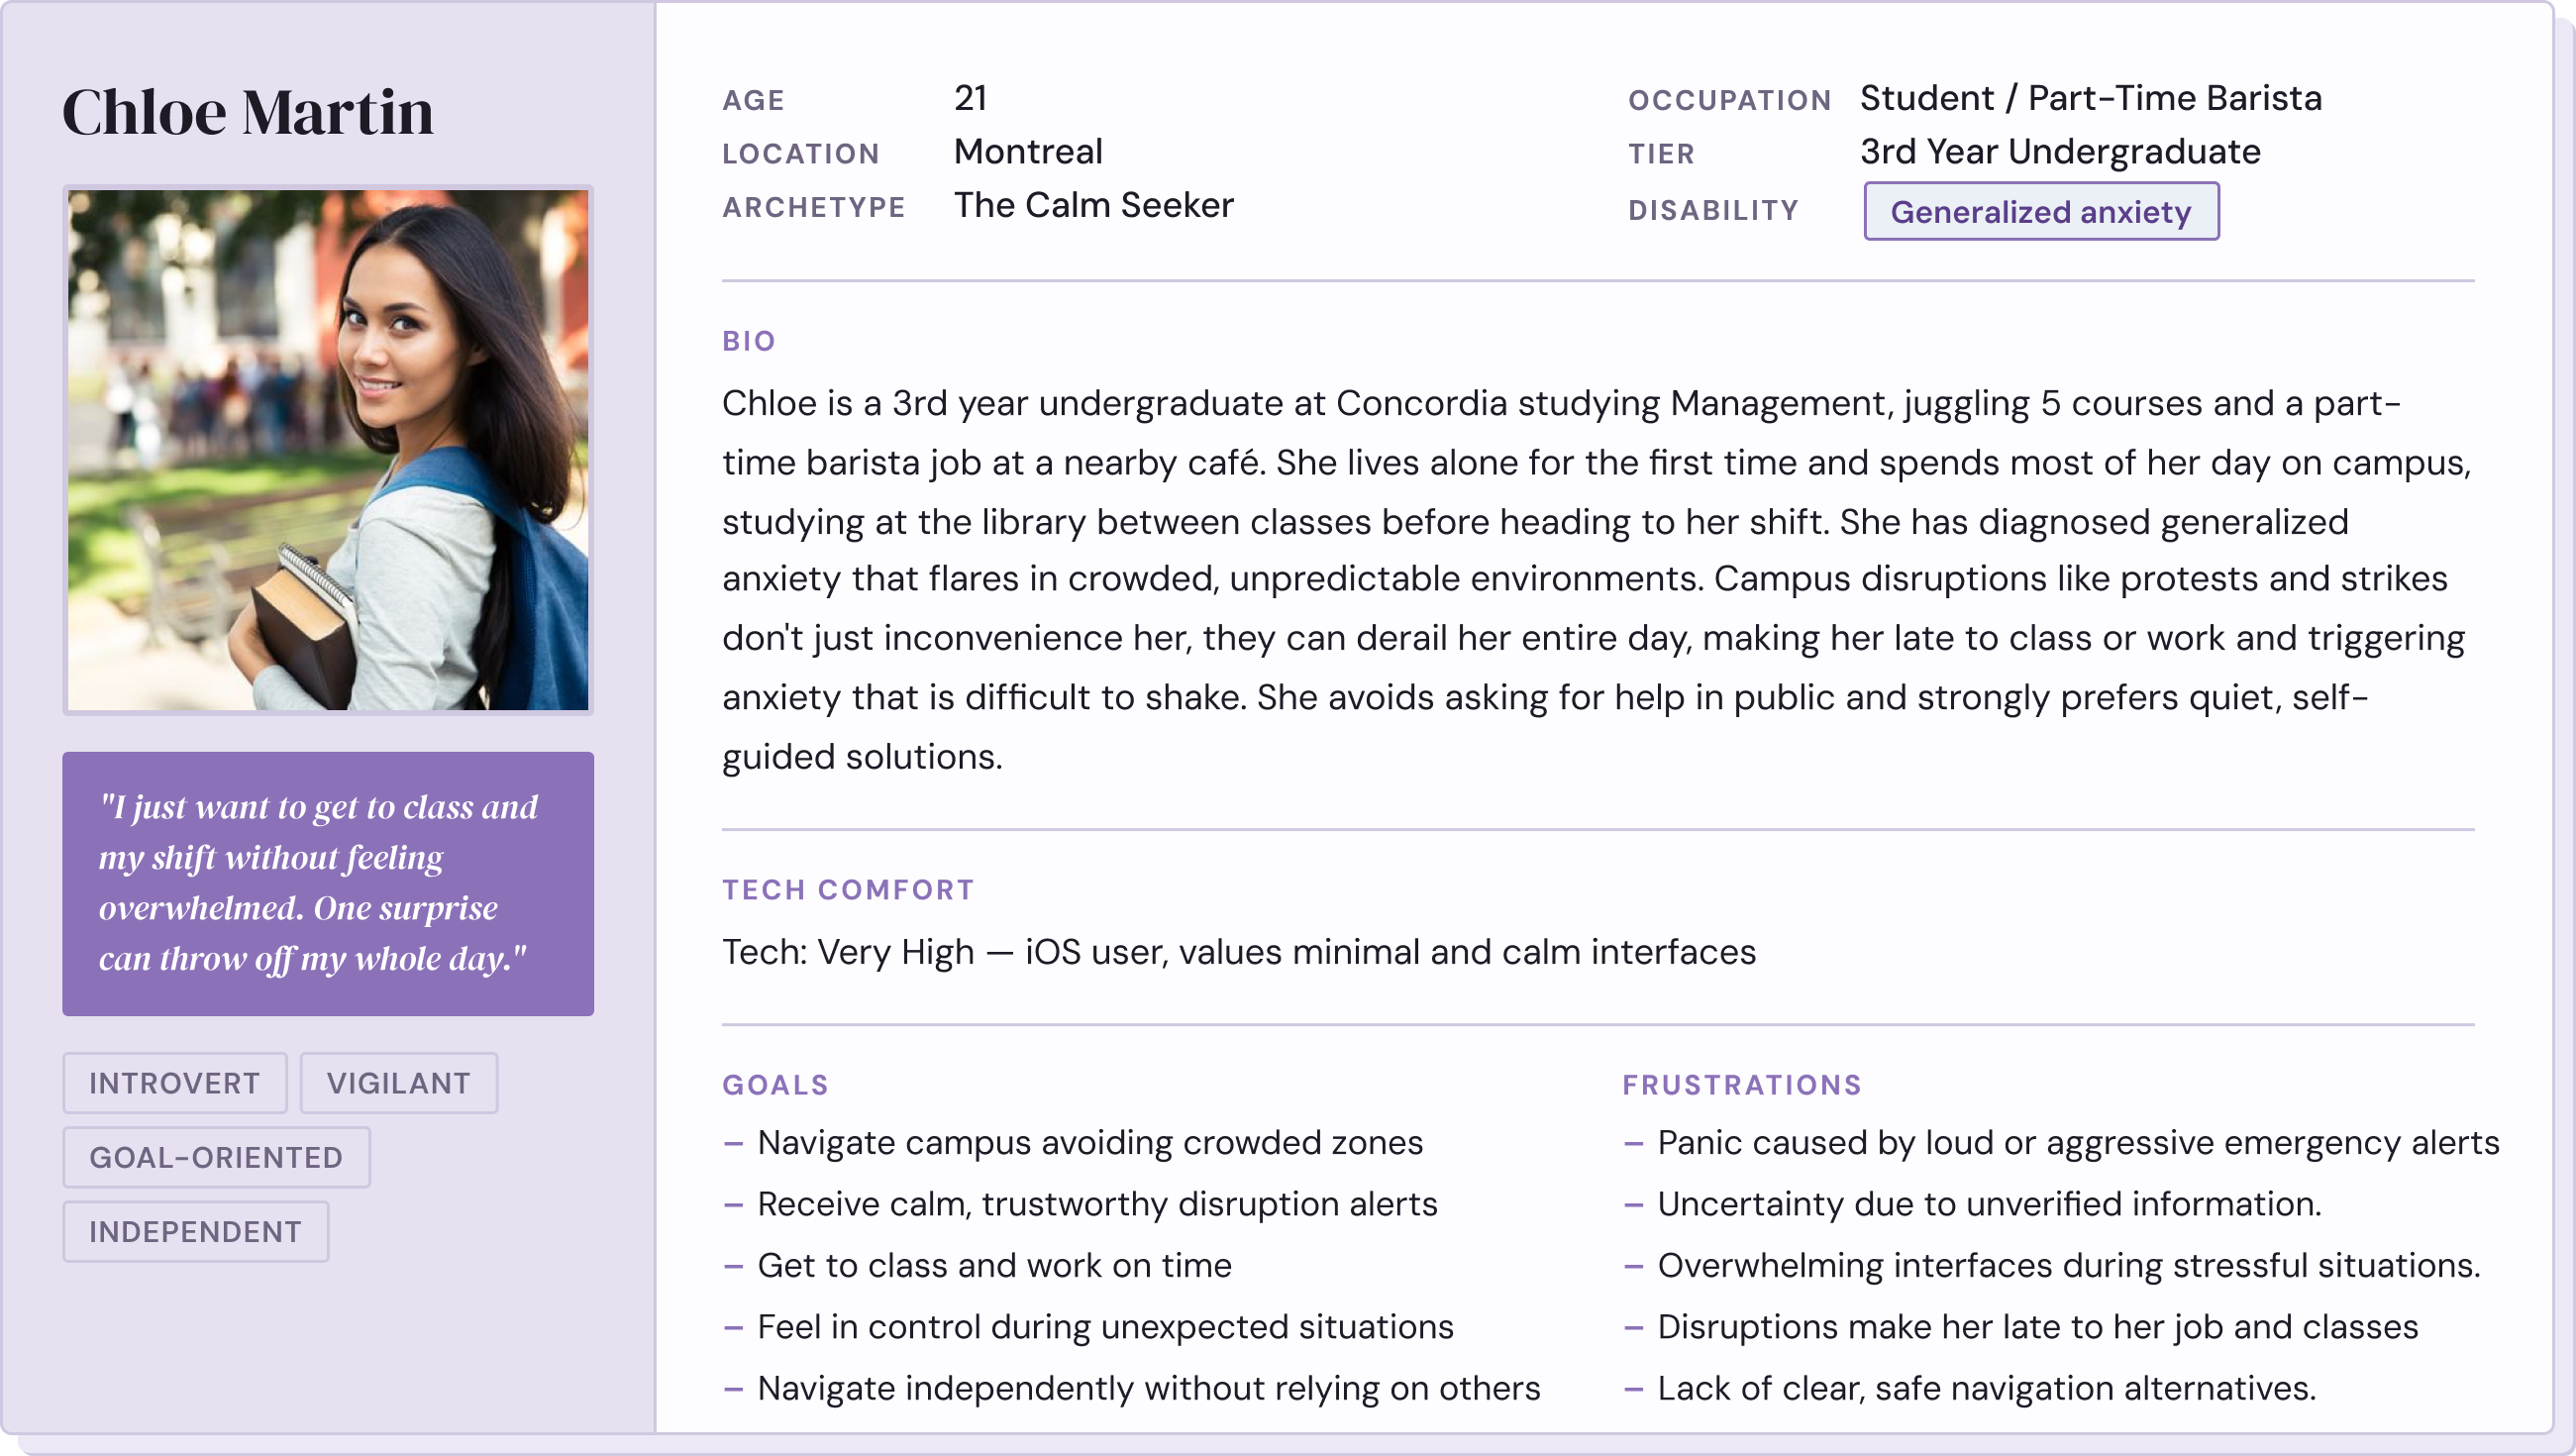
\includegraphics[width=\linewidth]{personas/ChloeMartin_Persona1.png}
  \caption{Persona 1: Chloe Martin --- Student with Generalized Anxiety.}
  \label{fig:persona_chloe}
\end{figure}
 
\begin{figure}[h]
  \centering
  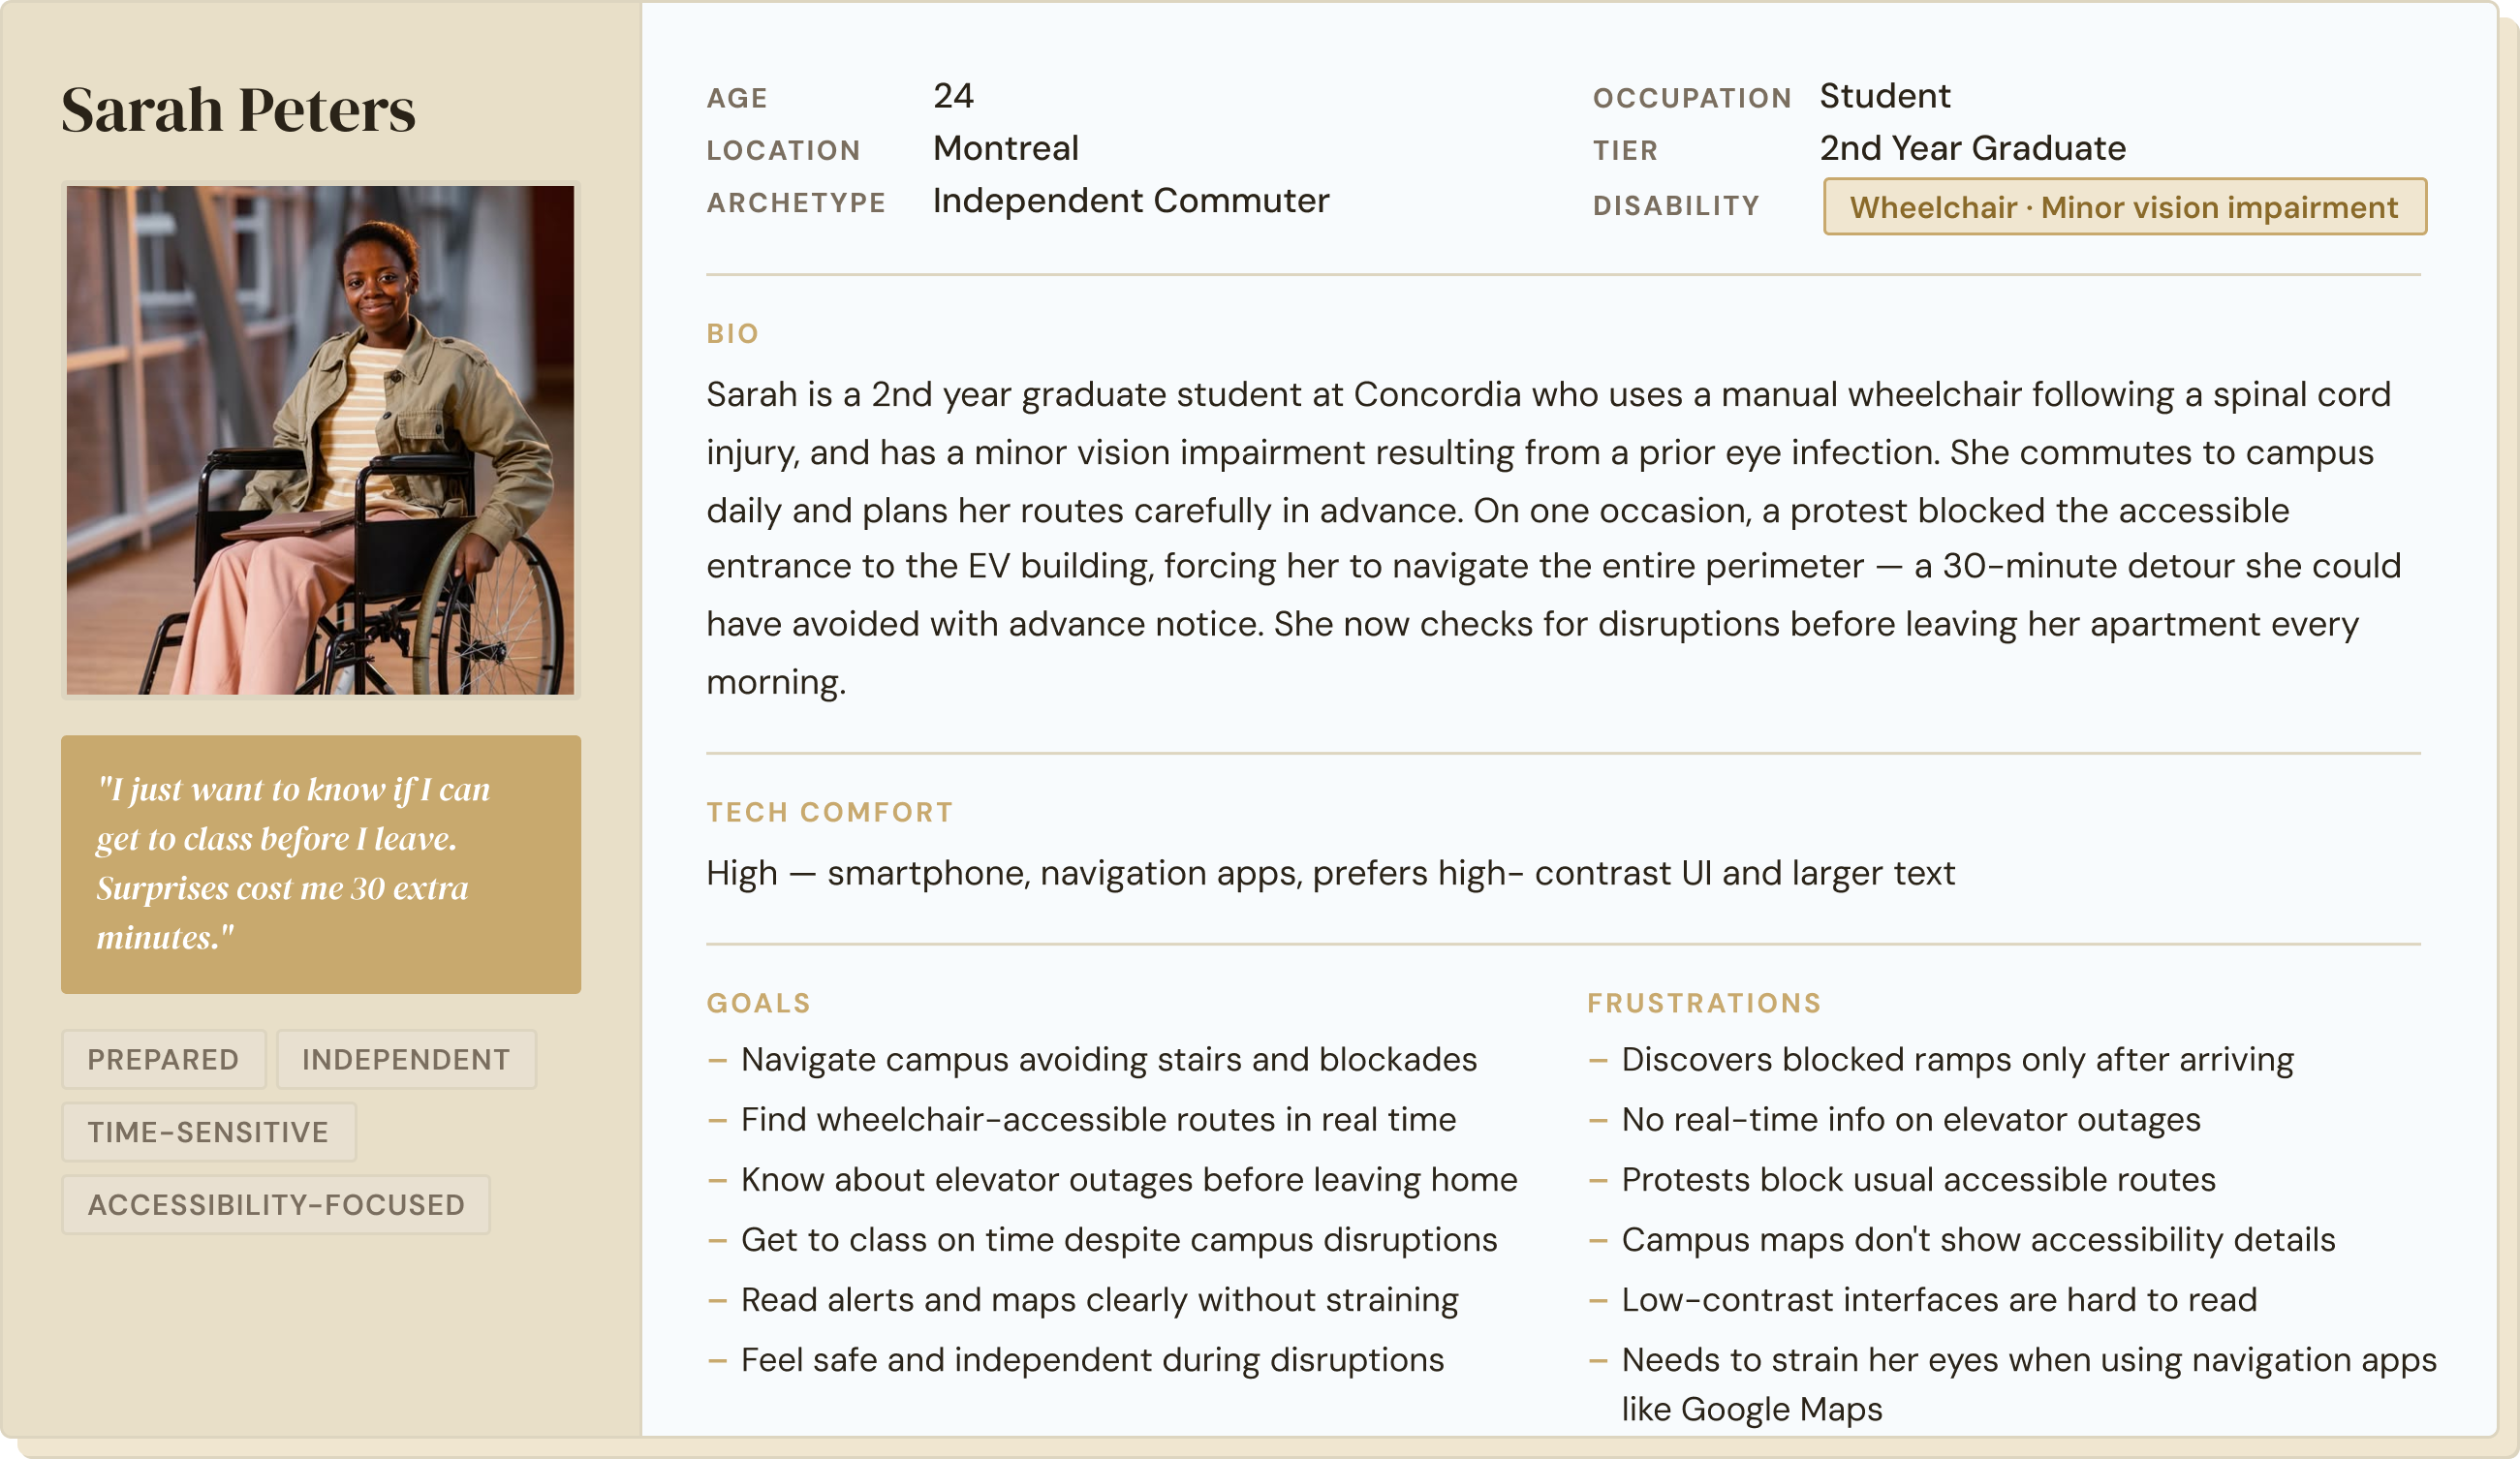
\includegraphics[width=\linewidth]{personas/SarahPeters_Persona2.png}
  \caption{Persona 2: Sarah Peters --- Student with Wheelchair and Minor Vision Impairment.}
  \label{fig:persona_sarah}
\end{figure}
 
\begin{figure}[h]
  \centering
  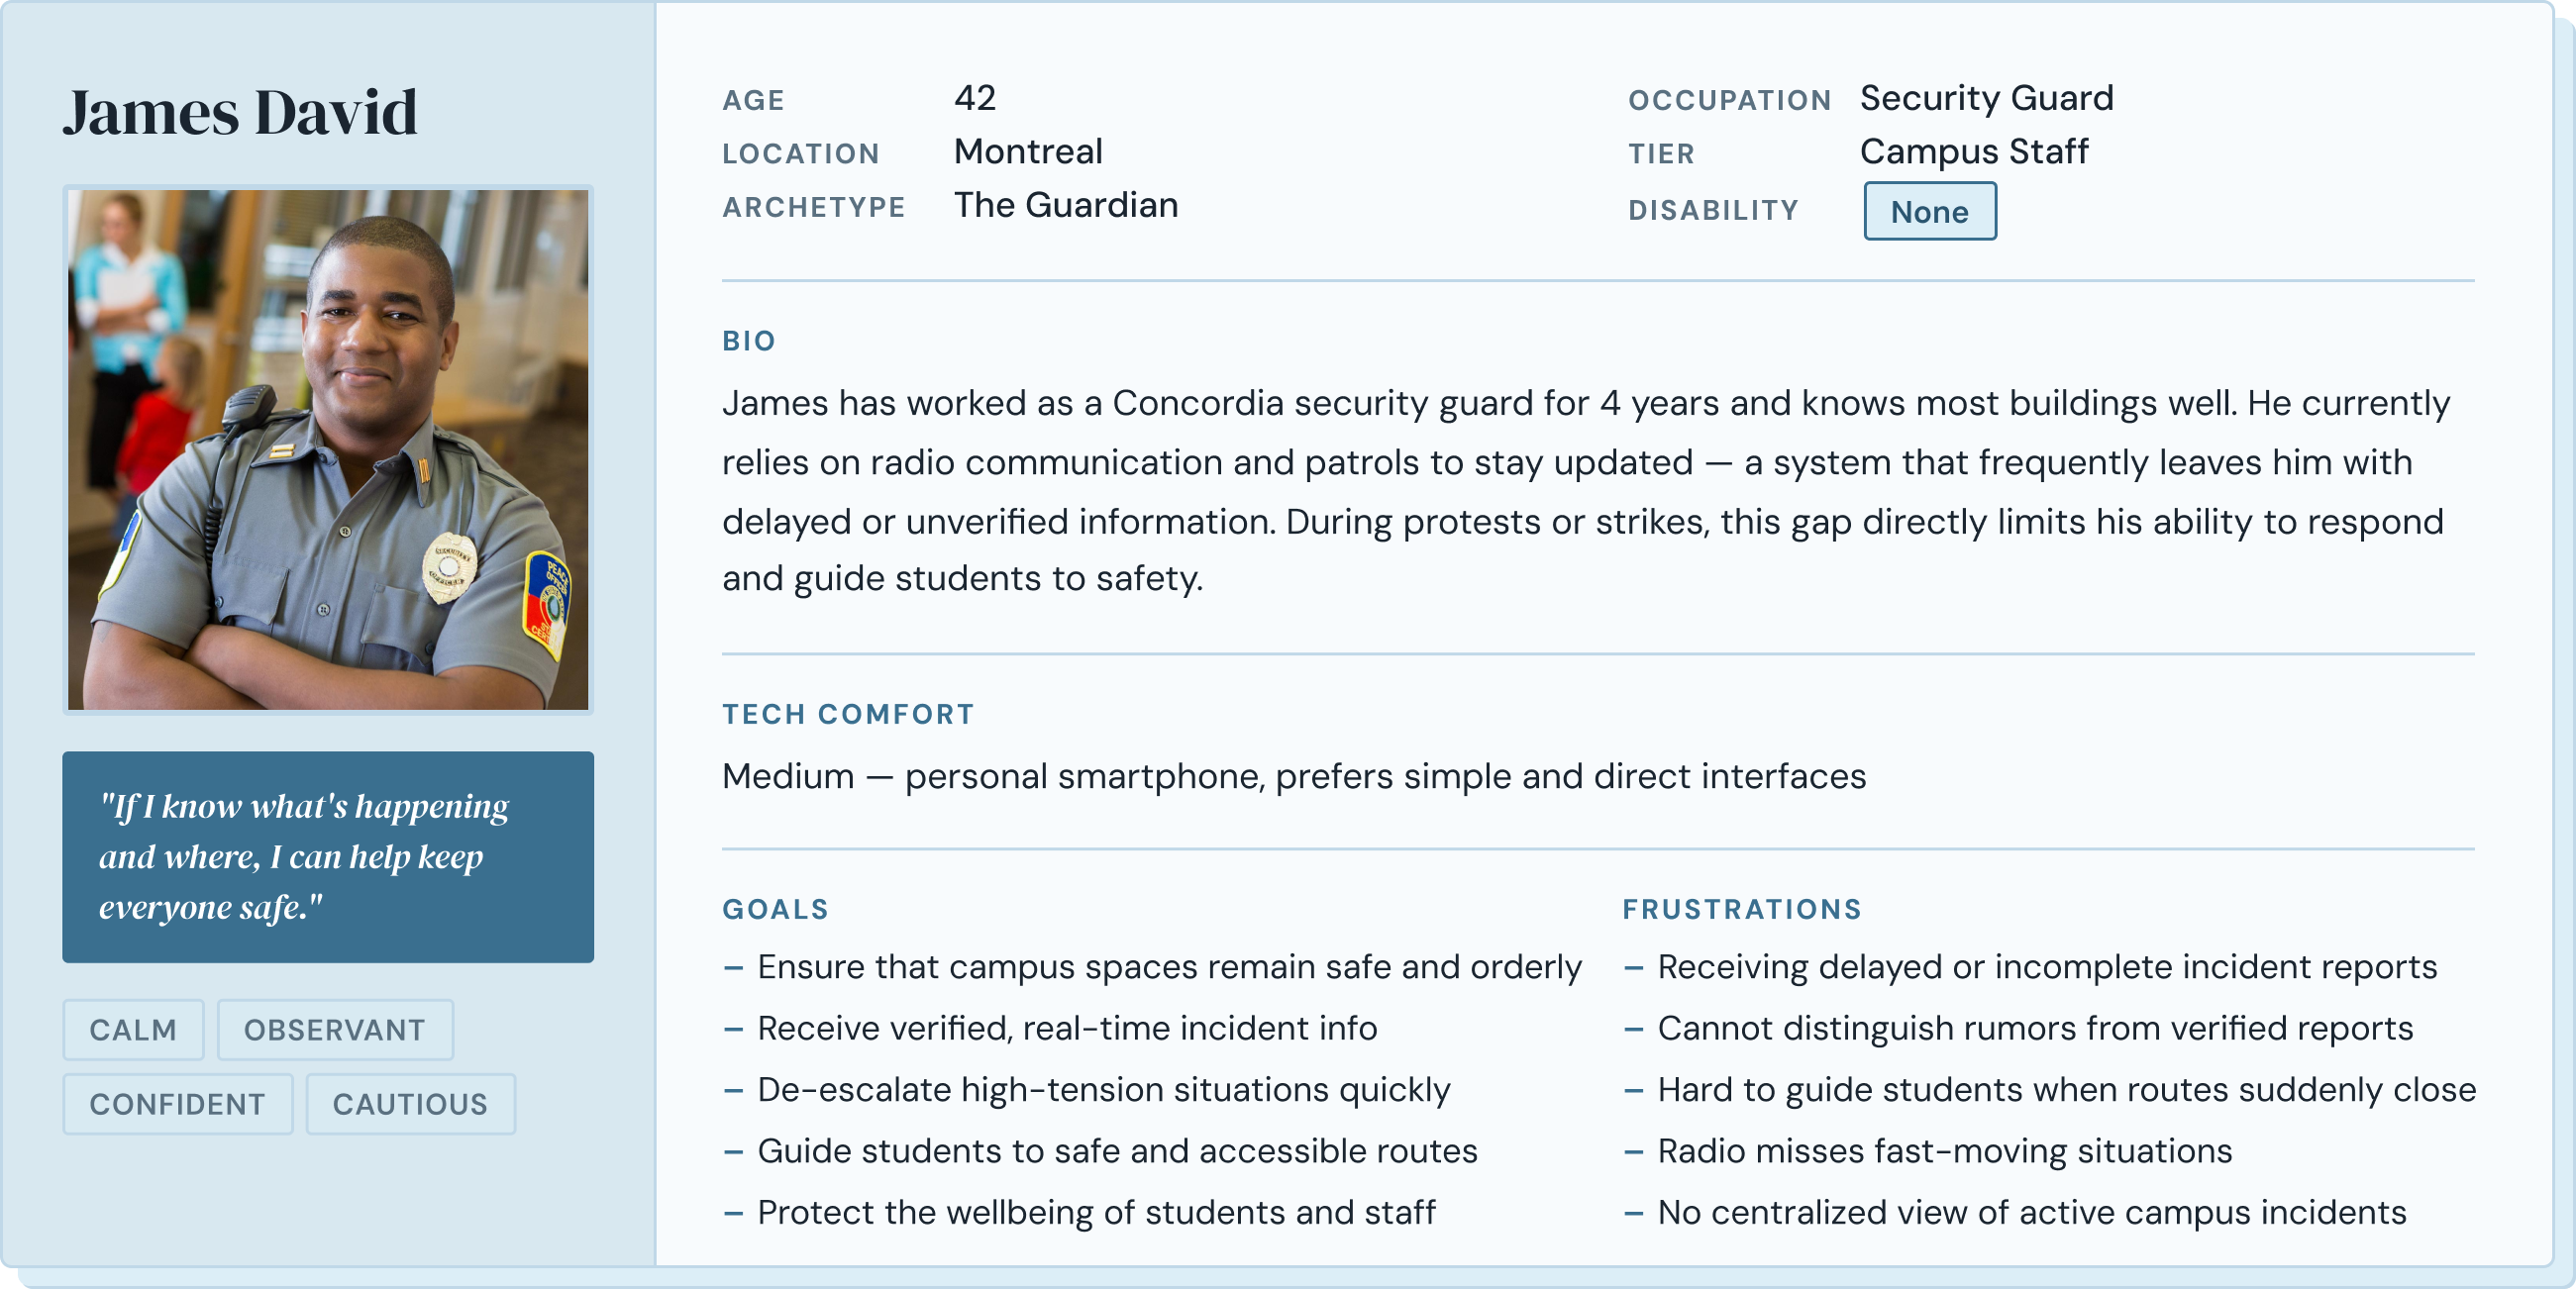
\includegraphics[width=\linewidth]{personas/JamesDavid_Persona3.png}
  \caption{Persona 3: James David --- Campus Security Staff.}
  \label{fig:persona_james}
\end{figure}
 
\subsection{Empathy Maps}
 
To move beyond the demographic and behavioral descriptions captured in our personas, we developed an empathy map for each persona~\cite{gray2017empathy}. For each persona, we mapped what the user \textit{thinks}, \textit{feels}, \textit{says}, and \textit{does} when navigating a campus disruption, as well as their core \textit{pains} and \textit{gains}. These maps were used to pressure-test our persona assumptions and to ensure that the system requirements defined in Section~\ref{sec:goals} are grounded in genuine user experience rather than assumed needs. Empathy maps for Chloe, Sarah, and James are shown in Figures~\ref{fig:empathy_chloe}, \ref{fig:empathy_sarah}, and~\ref{fig:empathy_james} respectively.
 
\begin{figure}[h]
  \centering
  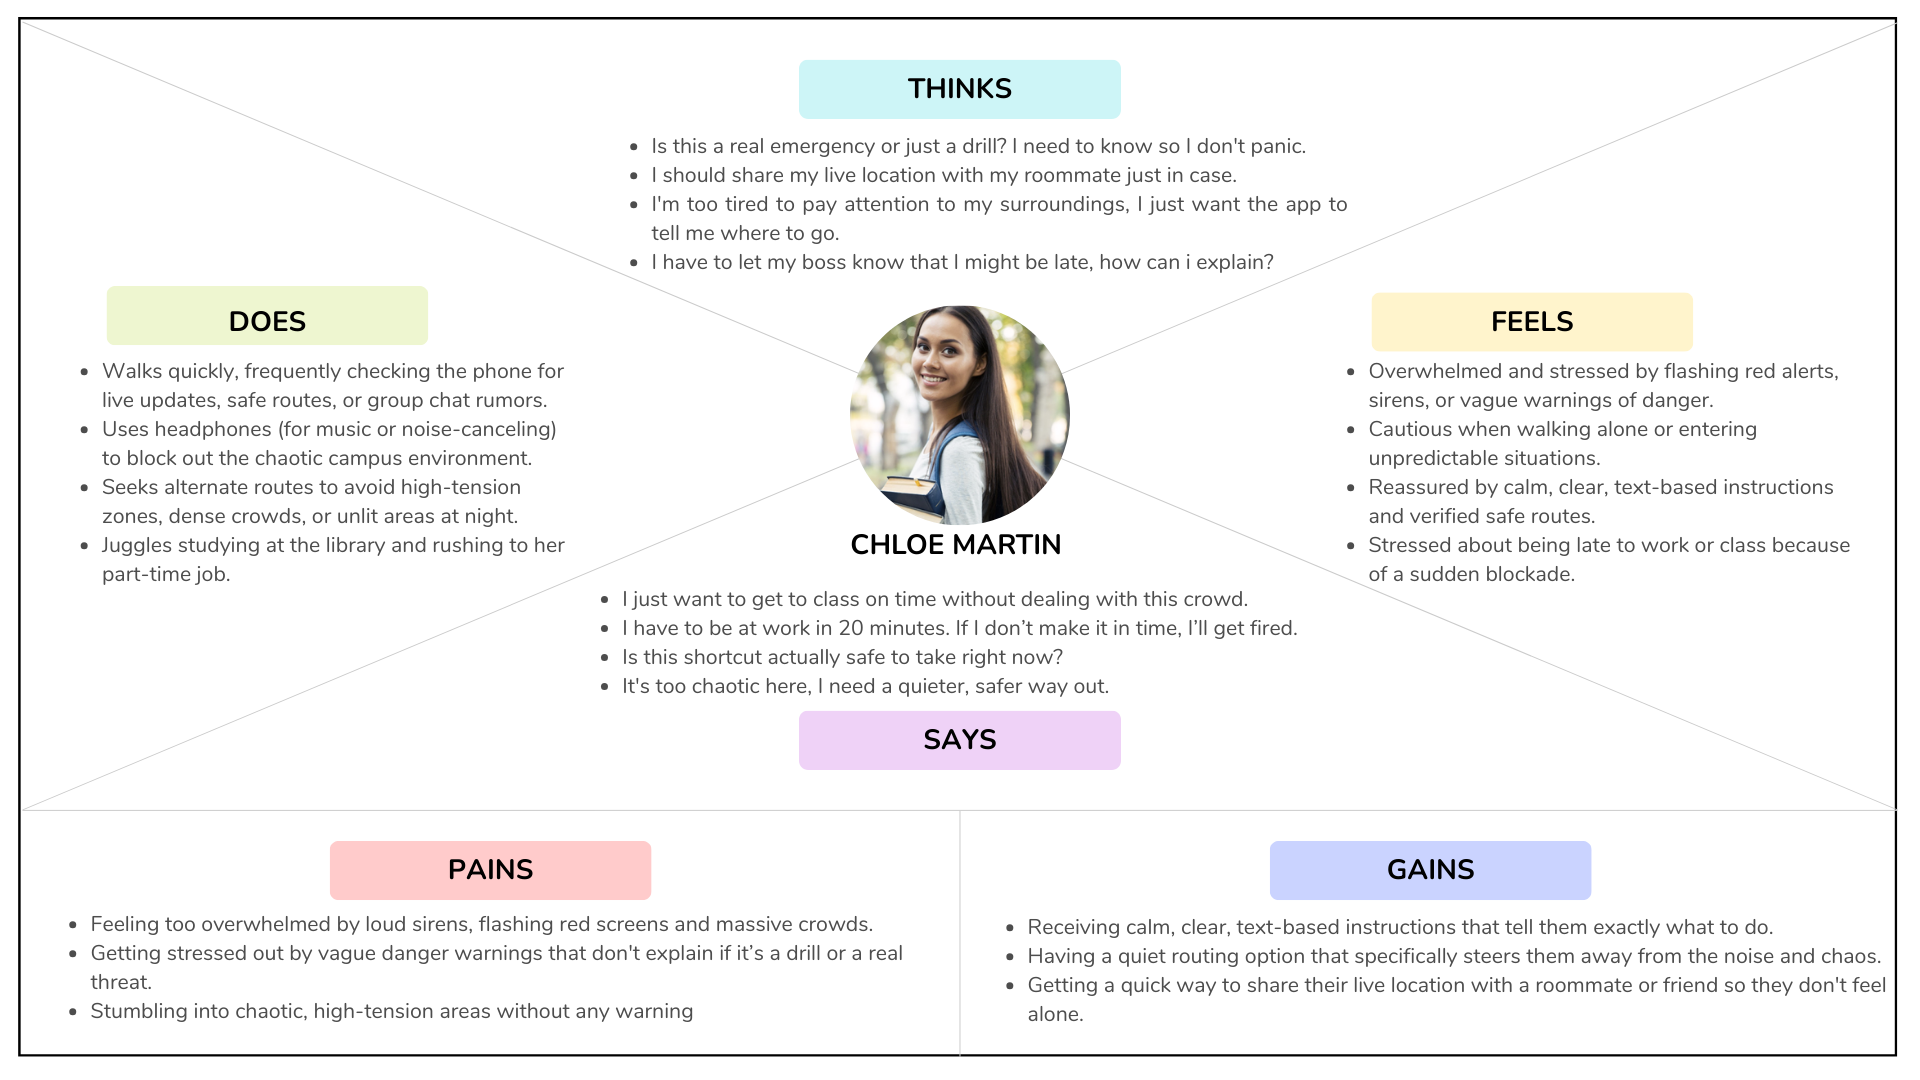
\includegraphics[width=\linewidth]{empathy_maps/chloe martin - empathy maps.png}
  \caption{Empathy Map: Chloe Martin --- Student with Generalized Anxiety.}
  \label{fig:empathy_chloe}
\end{figure}
 
\begin{figure}[h]
  \centering
  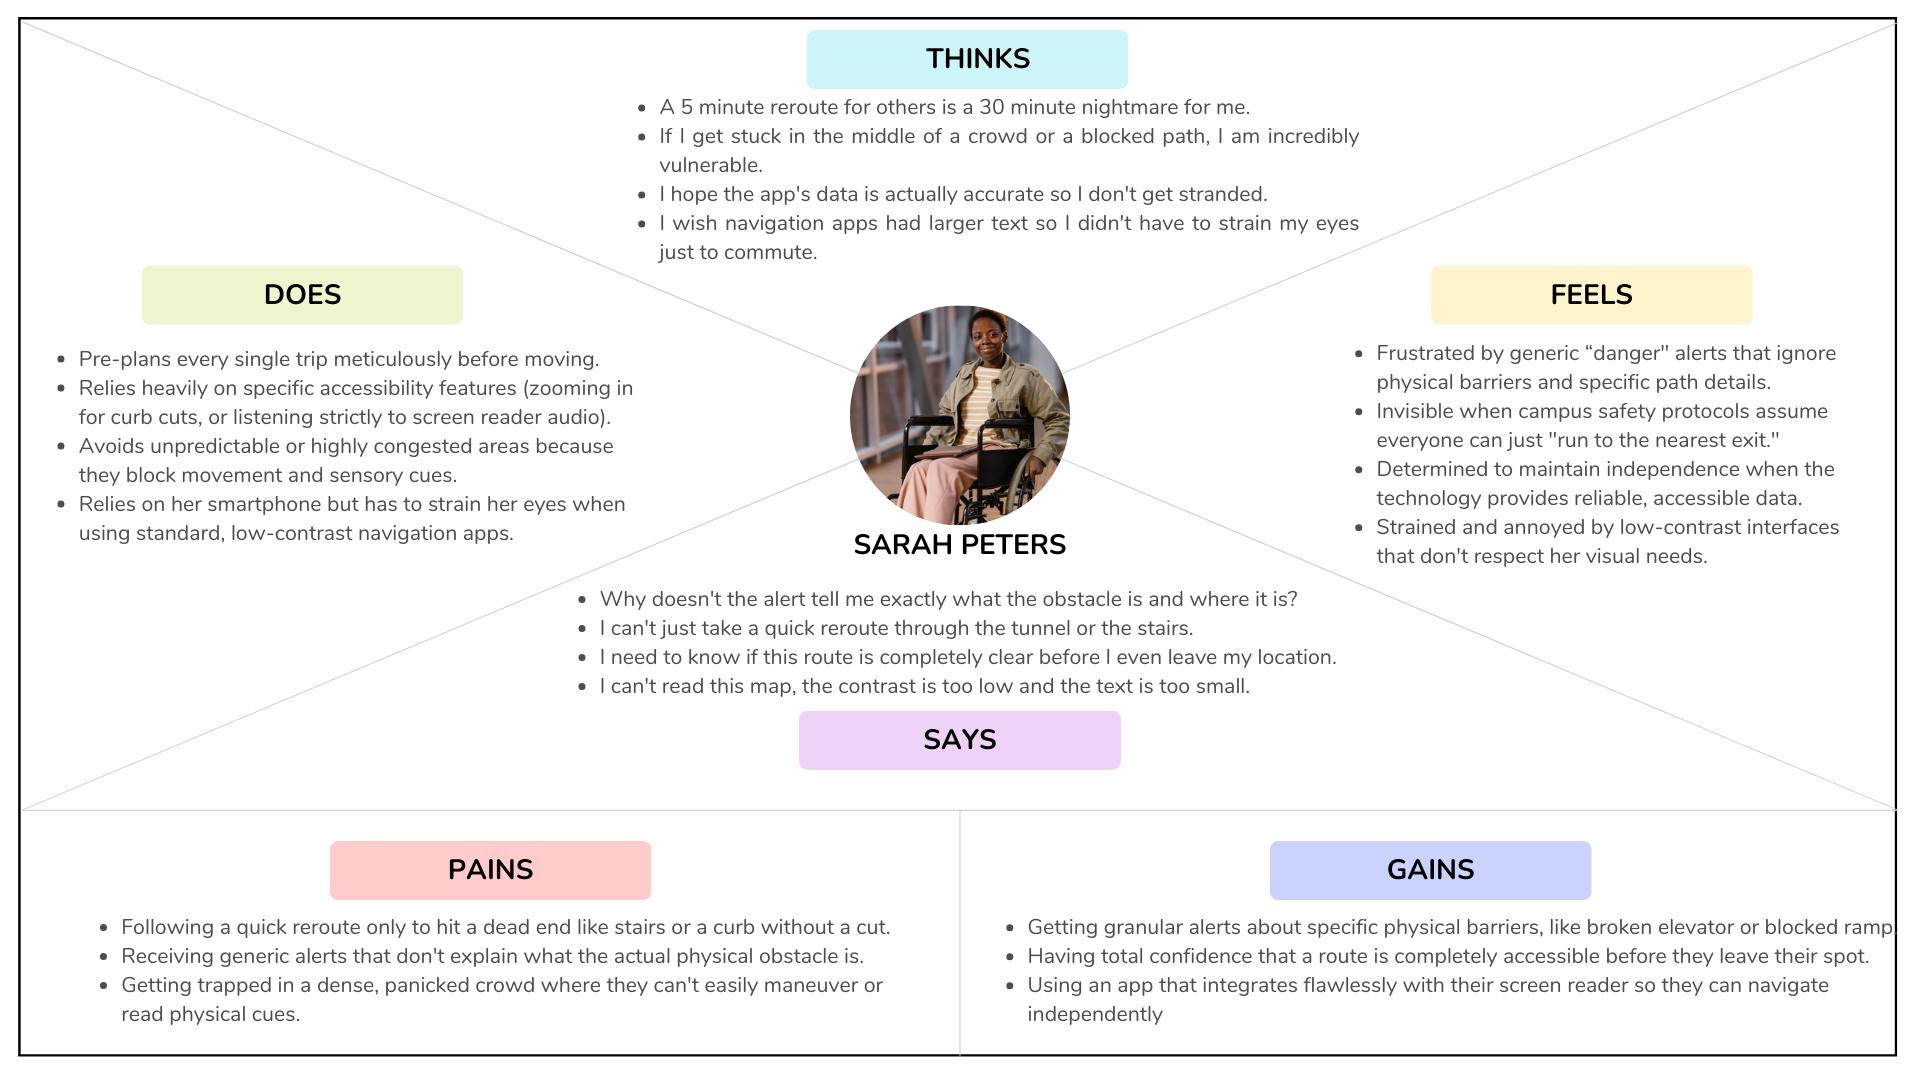
\includegraphics[width=\linewidth]{empathy_maps/sarah peters - empathy maps.png}
  \caption{Empathy Map: Sarah Peters --- Student with Wheelchair and Minor Vision Impairment.}
  \label{fig:empathy_sarah}
\end{figure}
 
\begin{figure}[h]
  \centering
  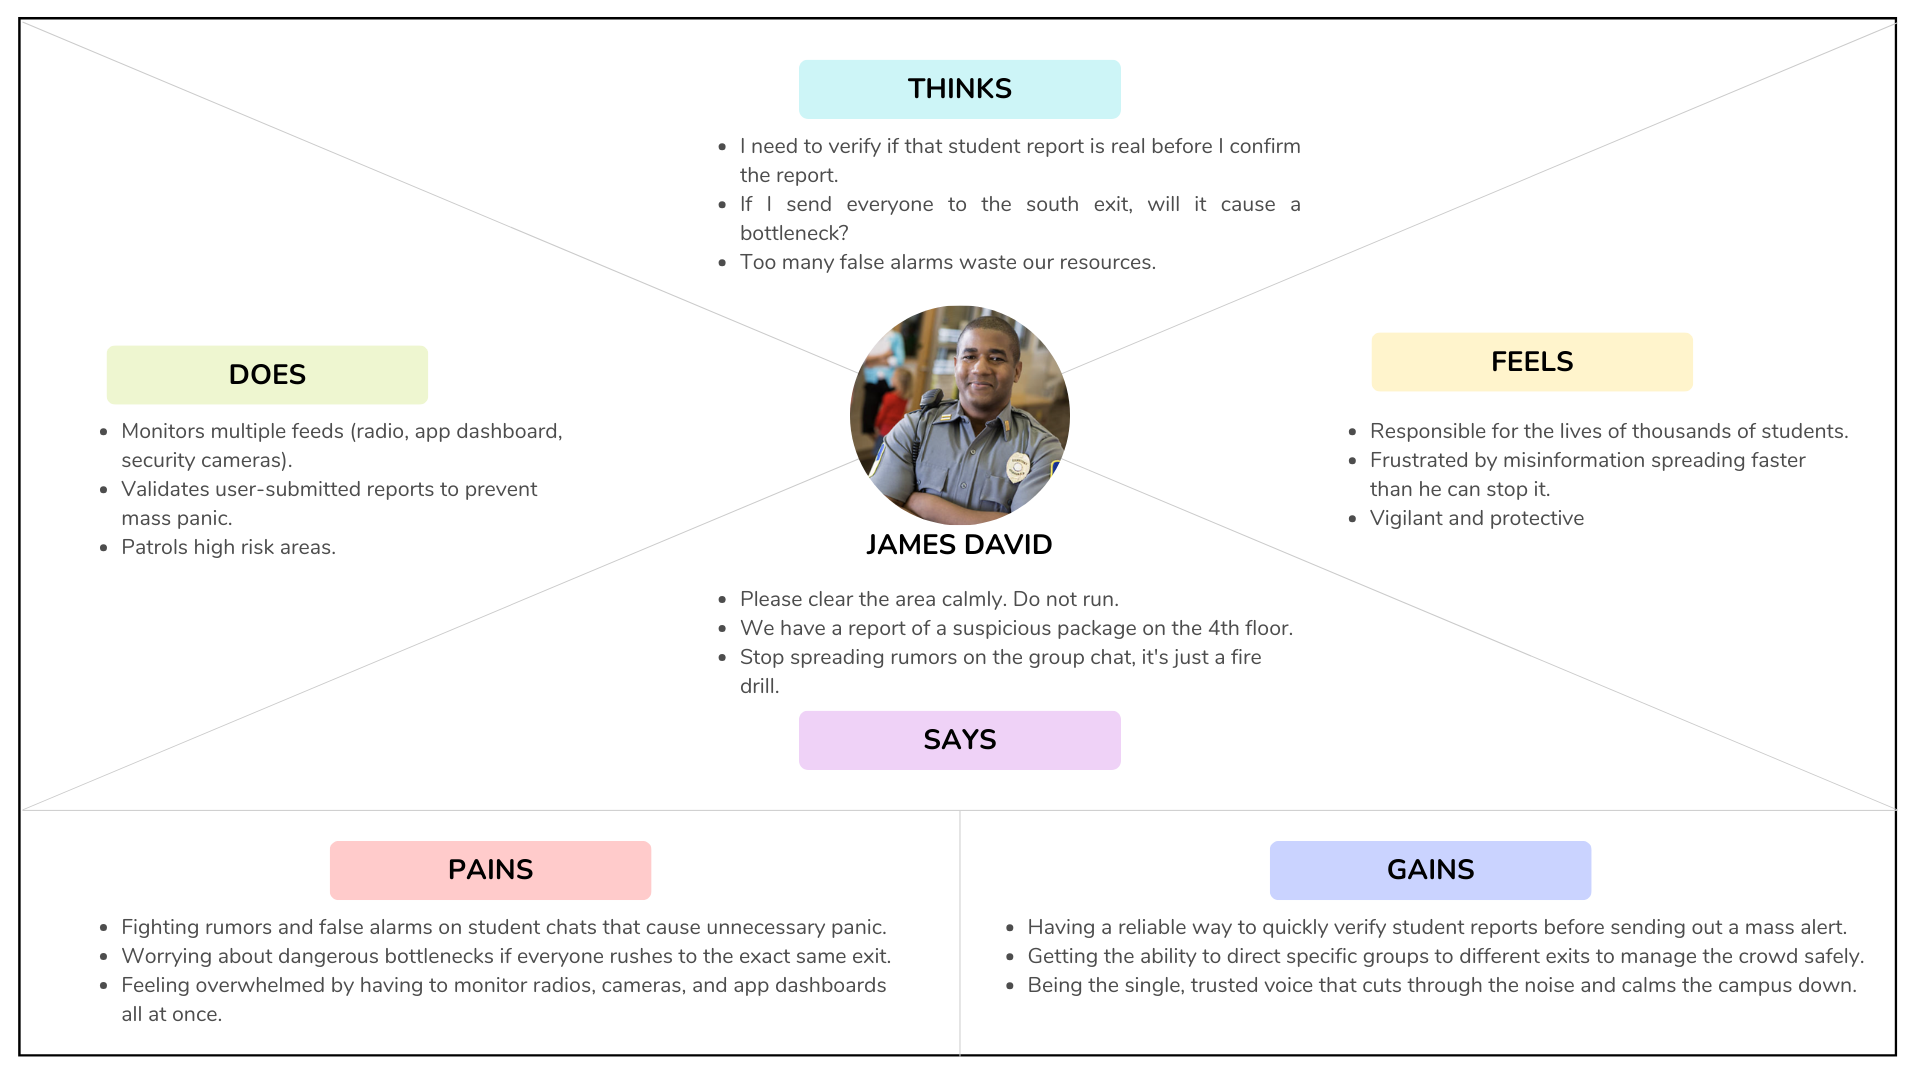
\includegraphics[width=\linewidth]{empathy_maps/james david - empathy maps.png}
  \caption{Empathy Map: James David --- Campus Security Staff.}
  \label{fig:empathy_james}
\end{figure}
 
\subsection{Journey Maps}
 
With a clear understanding of who our users are and how they experience the problem emotionally, journey maps were developed to trace each persona's end-to-end experience through a realistic campus disruption scenario. Journey maps plot a user's actions, thoughts, and emotional state across time~\cite{kalbach2016mapping}. Each journey map is tied to a concrete scenario relevant to Concordia's campus context.
 
\subsubsection*{Sarah Peters}
Sarah's scenario follows her morning commute to the EV building on a day when a protest has blocked her usual accessible entrance (see Figure~\ref{fig:journey_sarah} in Appendix~\ref{appendix:journeymaps}).
 
\subsubsection*{Chloe Martin}
Chloe's scenario follows her to work when she unexpectedly encounters a large, loud demonstration near the Hall building (see Figure~\ref{fig:journey_chloe} in Appendix~\ref{appendix:journeymaps}).
 
\subsubsection*{James David}
James's scenario follows his shift on a day when multiple incidents occur across campus and he must respond to them accordingly without any prior information (see Figure~\ref{fig:journey_james} in Appendix~\ref{appendix:journeymaps}).
 
These scenarios were chosen because they represent the most common and highest-impact disruption situations that our target users are likely to face, and because they expose the sharpest gaps between what users need and what existing tools currently provide. Together, the personas and journey maps form the foundation for the goal and task definitions in Section~\ref{sec:goals}, translating observed pain points into concrete system requirements.
 
\subsection{User Flow Diagrams}
\label{sec:prototyping}
 
Four user flow diagrams were developed to map how each persona moves through the application step by step. The Login / Sign Up flow (Figure~\ref{fig:flow_login}) covers account creation, role selection, and preference configuration. The Main Navigation flow (Figure~\ref{fig:flow_navigation}) shows how users move between core sections during a disruption. The Menu flow (Figure~\ref{fig:flow_menu}) covers access to emergency contacts, accessibility settings, and notification preferences. The Route Planning flow (Figure~\ref{fig:flow_route}) follows the steps a user takes to select a destination, review safe route options, and begin navigation. The full user flow diagrams are presented in Appendix~\ref{appendix:userflows}.
 
\subsection{Low-Fidelity Wireframes}
 
With the flows done, the next step was sketching out what the screens would actually look like. These wireframes are intentionally simple --- no colors, no images, just boxes and text to show where things go on each screen. Keeping it simple at this stage meant different layouts could be tried out quickly and decisions about structure could be made before spending time on the visual details. The full wireframes are presented in Appendix~\ref{appendix:lofi}.
 
\begin{itemize}[leftmargin=*, labelindent=0pt, itemsep=4pt]
    \item \textbf{Login / Sign Up} (Figure~\ref{fig:lofi_login}): covers the login screen, role selection, and the student and staff sign up screens.
    \item \textbf{Menu} (Figure~\ref{fig:lofi_menu}): covers the home page list view, hamburger menu variations, preferences setup, and the emergency resources screen.
    \item \textbf{Core UI Views} (Figure~\ref{fig:lofi_core}): covers the home page, map view, incident type selection, report incident view, incident detail view, and notification view.
\end{itemize}
 
\subsection{High-Fidelity Prototypes}
 
Although incorporating Concordia's burgundy, dark red, and gold tones was initially considered to reflect institutional identity, these colors are emotionally intense and commonly associated with urgency, danger, or alert states. In a safety-focused application for potentially stressful situations, such visually heavy tones could unintentionally heighten anxiety and may conflict with map indicators or warning signals, reducing visual clarity.
 
From a psychological and accessibility perspective, blue is better suited to our users. Blue is associated with calmness, trust, and stability, aligning with our goal of reducing stress during high-tension events. Additionally, red and green are most affected by color vision deficiency, whereas blue deficiency is extremely rare~\cite{birch1993practical}, making blue the most universally distinguishable and inclusive choice.
 
For these reasons, a two-tone monochromatic blue palette was selected: dark blue for headers and emphasis, and primary blue for buttons and interactive elements. Critical alert colors (red, yellow, green) are reserved strictly for status indicators to ensure they remain highly visible and meaningful. The color system also meets WCAG contrast ratio requirements, ensuring sufficient contrast between text and backgrounds for users with visual impairments.
 
To support cognitive comfort, the interface primarily uses white and off-white backgrounds. These neutral surfaces reduce visual noise and prevent overstimulation during prolonged use. Clear spacing between sections further enhances readability and reduces cognitive load.
 
Typography reinforces clarity and usability. Roboto was selected as the primary font because it is widely used in mobile apps, familiar to users, and optimized for mobile performance~\cite{google2014roboto}. Its readability and cross-platform compatibility reduce cognitive load and improve comfort. Body text is set at a minimum of 16px, secondary text at 14px, and headlines between 24--32px, in line with mobile UI best practices and WCAG recommendations~\cite{wcag21} for legibility and scalable text. Instead of pure black text, a dark grey tone is used to soften contrast while maintaining strong legibility.
 
Together, these design decisions create a calm, accessible, and visually clear interface aligned with the app's goal of supporting students safely and confidently during campus disruptions. The full high-fidelity prototypes are presented in Appendix~\ref{appendix:hifi}.
 
\begin{itemize}[leftmargin=*, labelindent=0pt, itemsep=4pt]
    \item \textbf{Login / Sign Up} (Figure~\ref{fig:hifi_login}): covers the login screen, role selection, student and staff sign up screens, and email confirmation.
    \item \textbf{Menu} (Figure~\ref{fig:hifi_menu}): covers the home page, hamburger menu, preferences setup, emergency resources screen, and profile page.
    \item \textbf{Core UI Views} (Figure~\ref{fig:hifi_core}): covers the home page, filtered list view, map view, incident reporting, incident detail views, notifications screen, and confirmation pop-up.
    \item \textbf{Route Planning} (Figure~\ref{fig:hifi_route}): covers the accessibility filter screen, route preview, suggested action view, and safe zone button state.
\end{itemize}
%%
%% 4. SYSTEM FUNCTIONALITY
%%
\section{System Functionality}
\label{sec:functionality}
 
The screens in this section show the final product of the design process outlined in Section 3. They are screenshots taken straight from the working Android application. The layout, color scheme, typography, and interaction patterns were all faithfully translated from design into code using the high-fidelity Figma prototypes. The basic design rationale such as calm technology, WCAG AA compliance, and less cognitive load, remained the guiding concept when implementation restrictions required modifications.
 
Concordia Safe Path is a cross-platform mobile application targeting Android that uses React Native and ExpoRouter. Expo Router provides a file-based navigation architecture suited to the multi-screen structure of the system. The backend is powered by Supabase, which provides real-time database capabilities, user authentication, and storage built on PostgreSQL. RowLevel Security (RLS) policies enforce role-based access control at the database level, ensuring that staff-only actions such as incident verification cannot be performed by student accounts at the API level. Campus map rendering, routing, and incident visualization are handled with the Google Maps SDK via the react-native-maps library. Production builds are distributed as APKs via EAS Build.
 
Development process followed standard software engineering practices throughout this project. The codebase is hosted on GitHub at https://github.com/luantran/concordia-safe-path, with all feature work carried out on dedicated branches and integrated into the main branch exclusively through pull requests. Each pull request required a written description, screenshots of affected screens, and at least one team member toreview before merging with the working code. Using the same pull request template enforced consistency across contributions and made it easier to review new code.  Work was tracked using GitHub Projects with a Kanban board, allowing the team to coordinate tasks between the members and maintain visibility into what was in progress, under review, and complete. This workflow ensured that the codebase remained stable and reviewable at every stage of development by any member. 
\subsection{Authentication and Onboarding}
 
\begin{figure}[H]
  \centering
  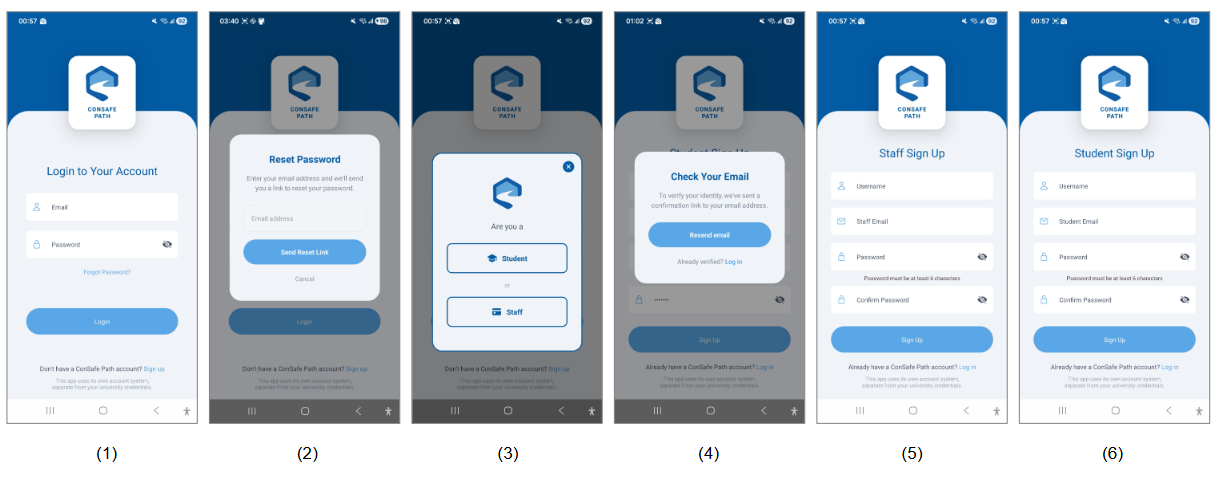
\includegraphics[width=\columnwidth, keepaspectratio]{screenshots/authentication.png}
  \caption{Authentication screens: (1) login, (2) password reset, (3) role selection, (4) email verification, (5) staff sign up, (6) student sign up.}
  \label{fig:auth}
\end{figure}
 
The authentication flow (Figure~\ref{fig:auth}) supports account creation for both students and staff, with role selection at sign-up determining permissions throughout the app. Staff accounts gain access to verification and resolution controls not available to students. This addresses \textbf{Goal 1}.
 
\subsection{Preferences and Accessibility Settings}
 
\begin{figure}[H]
  \centering
  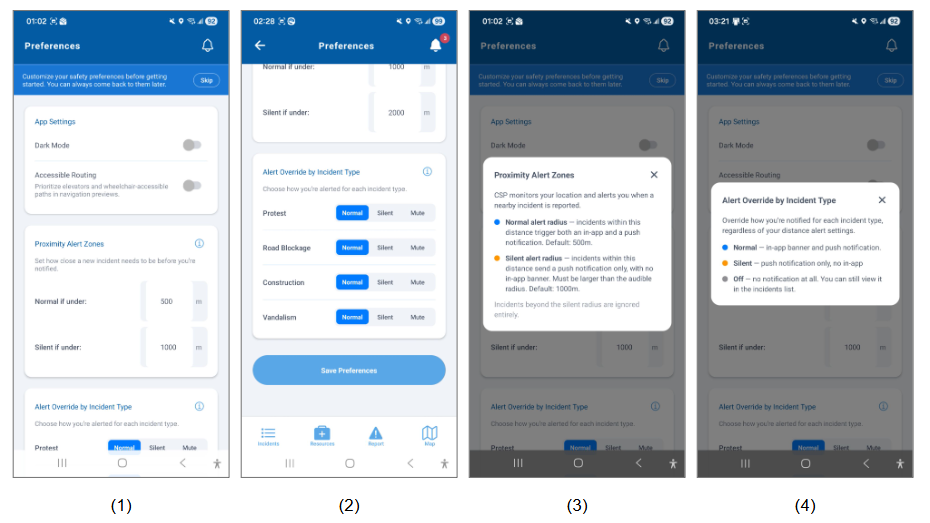
\includegraphics[width=\columnwidth, keepaspectratio]{screenshots/preferences.png}
  \caption{Preferences screens: (1) main preferences with onboarding banner, (2) alert distance and incident type override settings, (3) proximity alert zone info modal, (4) alert override by incident type info modal.}
  \label{fig:preferences}
\end{figure}
 
The preferences screen (Figure~\ref{fig:preferences}) allows users to configure accessible routing, proximity alert distances, and per-incident-type notification behavior (Normal, Silent, or Mute). An onboarding banner guides first-time users through setup without blocking access. This addresses \textbf{Goal 1} and \textbf{Goal 10}.
 
\subsection{Campus Map and Incident Visualization}
 
\begin{figure}[H]
  \centering
  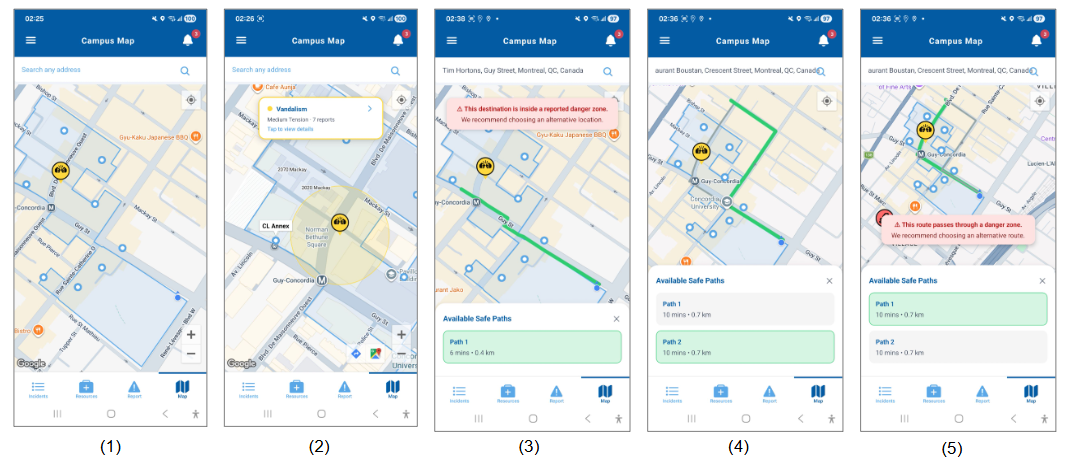
\includegraphics[width=\columnwidth, keepaspectratio]{screenshots/map_and_routes.png}
  \caption{Map screens: (1) live incident map, (2) incident callout with building markers, (3) danger zone warning on destination, (4) safe route options, (5) route passing through danger zone warning.}
  \label{fig:map}
\end{figure}
 
The map screen (Figure~\ref{fig:map}) shows live color-coded incident markers across the SGW campus. When a user enters a destination, the system warns if it falls within a danger zone and flags any route passing through one. Multiple route options are shown with time and distance estimates. This addresses \textbf{Goals 2}, \textbf{6}, and \textbf{8}.
 
\subsection{Proximity Alerts and Safe Zone}
 
\begin{figure}[H]
  \centering
  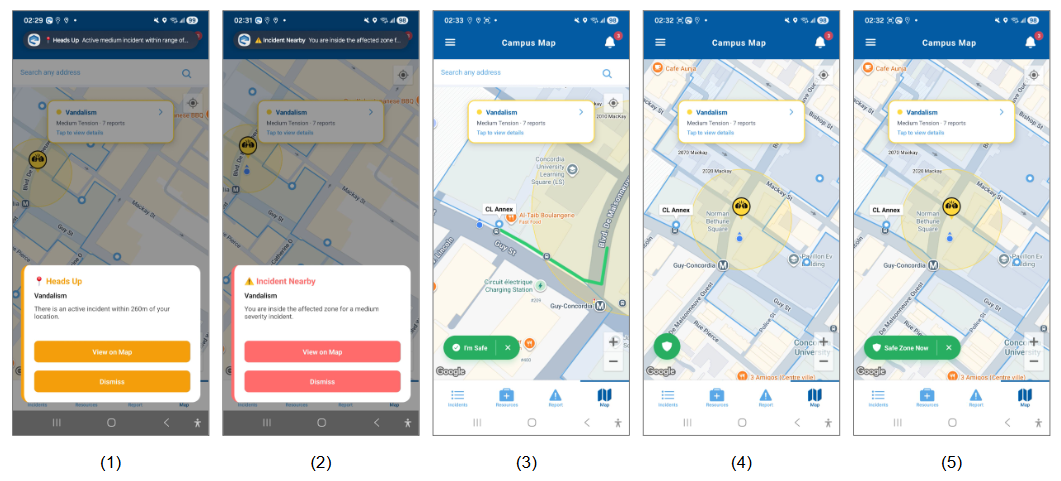
\includegraphics[width=\columnwidth, keepaspectratio]{screenshots/proximity.png}
  \caption{Proximity alert screens: (1) level 1 ``Heads Up'' alert, (2) level 2 ``Incident Nearby'' alert, (3) safe route displayed after entering danger zone, (4) ``I'm Safe'' confirmation state, (5) ``Safe Zone Now'' persistent button.}
  \label{fig:proximity}
\end{figure}
 
The proximity alert system (Figure~\ref{fig:proximity}) triggers progressive alerts as users approach an incident zone: a ``Heads Up'' banner at the outer radius, escalating to an ``Incident Nearby'' modal at the inner zone. A persistent ``Safe Zone Now'' button remains visible until the user confirms they are safe. This implements graduated escalation from \textbf{Goal 6} and one-touch safe zone access from \textbf{Goal 2}.
 
\subsection{Incident Reporting}
 
\begin{figure}[H]
  \centering
  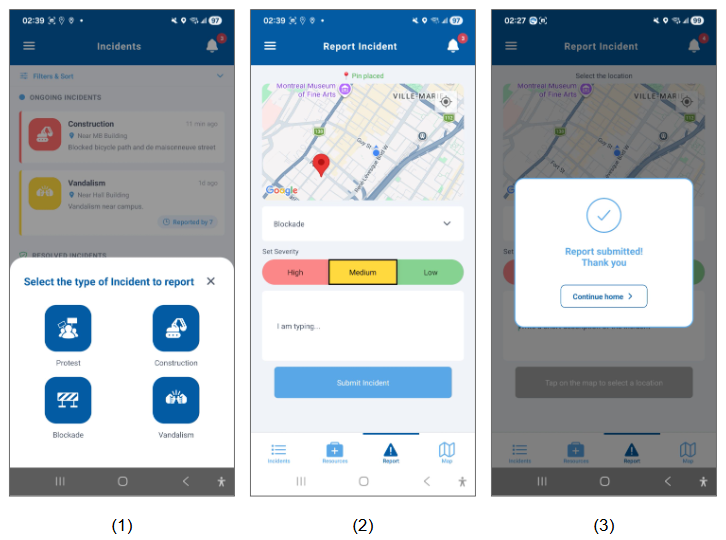
\includegraphics[width=\columnwidth, keepaspectratio]{screenshots/reporting.png}
  \caption{Incident reporting screens: (1) incident type selection modal, (2) report form with map pin, severity selector, and description field, (3) submission confirmation.}
  \label{fig:reporting}
\end{figure}
 
Incident reporting (Figure~\ref{fig:reporting}) is reachable in one tap from any screen. Users select an incident type, place a pin or use their current location, set severity, and optionally add a description. A confirmation is shown on submission. The severity selector uses color alongside text labels for accessibility. This addresses \textbf{Goals 7} and \textbf{10}.
 
\subsection{Incident List and Detail View}
 
\begin{figure}[H]
  \centering
  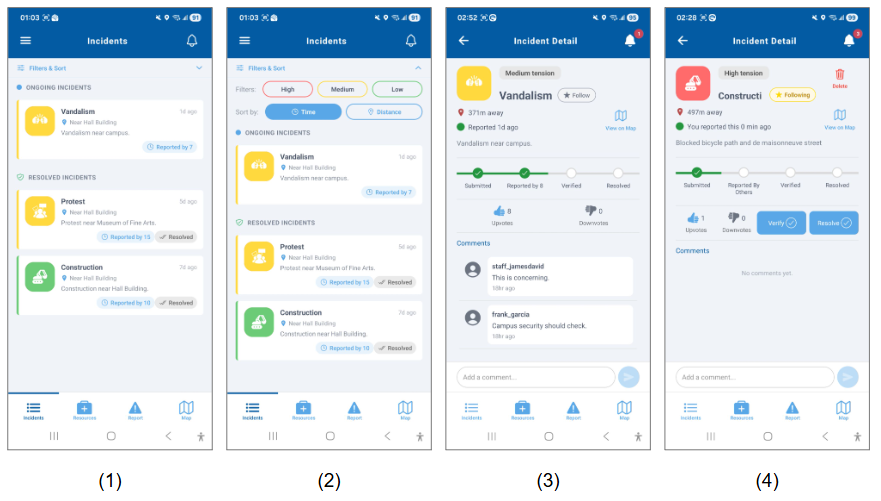
\includegraphics[width=\columnwidth, keepaspectratio]{screenshots/incident-detail-list.png}
  \caption{Incident list and detail screens: (1) list view with ongoing and resolved sections, (2) filtered and sorted list view, (3) student incident detail with verification progress, upvotes, and comments, (4) staff incident detail with verify and resolve controls.}
  \label{fig:incidents}
\end{figure}
 
The incident list (Figure~\ref{fig:incidents}) groups reports into ongoing and resolved sections with color-coded severity and verification badges, filterable by severity and sortable by time or distance. The detail view shows a four-stage verification progress bar, upvote and downvote counts, a follow button, and a comments section. Staff accounts see Verify and Resolve controls. This addresses \textbf{Goals 1}, \textbf{3}, and \textbf{4}.
 
\subsection{Notifications and Offline Mode}
 
\begin{figure}[H]
  \centering
  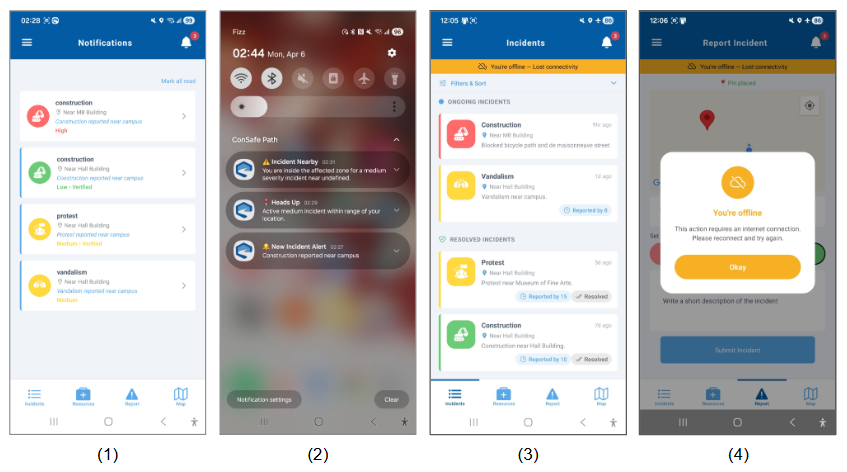
\includegraphics[width=\columnwidth, keepaspectratio]{screenshots/notifications_and_offline.png}
  \caption{Notifications and offline screens: (1) in-app notifications list, (2) system push notifications on the device lock screen, (3) offline banner with reduced-functionality incident list, (4) offline modal blocking actions that require connectivity.}
  \label{fig:notifications}
\end{figure}
 
The notifications screen (Figure~\ref{fig:notifications}) logs all received alerts. Push notifications are delivered even when the app is backgrounded. When offline, a persistent banner appears on every screen and actions requiring connectivity display an explanatory modal rather than failing silently. Cached data remains visible in read-only state. This addresses \textbf{Goals 2}, \textbf{5}, and \textbf{6}.
 
\subsection{Menu, Emergency Resources, and Profile}
 
\begin{figure}[H]
  \centering
  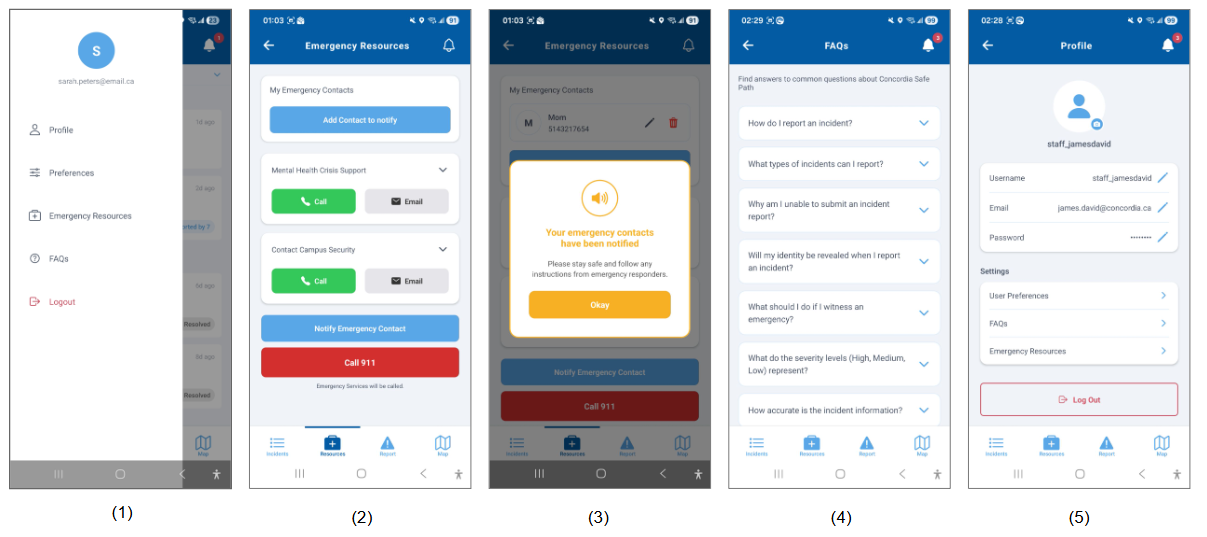
\includegraphics[width=\columnwidth, keepaspectratio]{screenshots/menu.png}
  \caption{Menu and support screens: (1) hamburger menu with navigation links, (2) emergency resources with contact options, (3) emergency contact notification confirmation, (4) FAQs accordion, (5) profile page with editable user details.}
  \label{fig:menu}
\end{figure}
 
The menu (Figure~\ref{fig:menu}) provides access to preferences, emergency resources, FAQs, and the profile page. The emergency resources screen offers one-tap call and email buttons for mental health support and campus security, a ``Notify Emergency Contact'' button, and a prominently placed ``Call 911'' button. This addresses \textbf{Goals 9} and \textbf{10}.
 
%%
%% 5. EVALUATION OF EXISTING SYSTEMS
%%
\section{Evaluation of Existing Systems}
\label{sec:background}
 
As part of our problem space investigation, we surveyed five existing mobile safety applications --- Rave Guardian, LiveSafe, Citizen, Life360, and AccessNow --- to understand the current landscape and identify the gaps that motivate the design of CSP. Table~\ref{tab:comparison} summarizes the key features of each surveyed application compared to Concordia Safe Path.
 
\begin{table}[H]
\centering
\caption{Feature comparison of existing safety applications and Concordia Safe Path.}
\label{tab:comparison}
\renewcommand{\arraystretch}{1.3}
\setlength{\tabcolsep}{4pt}
\begin{tabular}{|M{0.22\linewidth}|c|c|c|c|c|c|}
\hline
\rowcolor{tableheader}
\textcolor{white}{\textbf{Feature}}
  & \textcolor{white}{\textbf{\rotatebox{60}{Rave G.}}}
  & \textcolor{white}{\textbf{\rotatebox{60}{Citizen}}}
  & \textcolor{white}{\textbf{\rotatebox{60}{LiveSafe}}}
  & \textcolor{white}{\textbf{\rotatebox{60}{Life360}}}
  & \textcolor{white}{\textbf{\rotatebox{60}{AccessNow}}}
  & \textcolor{white}{\textbf{\rotatebox{60}{CSP}}} \\
\hline
\rowcolor{tablerowA}
Real-time alerts          & \checkmark & \checkmark & \checkmark &            &            & \checkmark \\
\hline
\rowcolor{tablerowB}
User-reported incidents   &            & \checkmark & \checkmark &            &            & \checkmark \\
\hline
\rowcolor{tablerowA}
Emergency contact         & \checkmark & \checkmark & \checkmark & \checkmark &            & \checkmark \\
\hline
\rowcolor{tablerowB}
Danger zone visualisation &            & \checkmark &            &            &            & \checkmark \\
\hline
\rowcolor{tablerowA}
Calm tech design          &            &            &            &            &            & \checkmark \\
\hline
\rowcolor{tablerowB}
Accessibility features    &            &            &            &            & \checkmark & \checkmark \\
\hline
\rowcolor{tablerowA}
Safe route navigation     &            &            &            &            &            & \checkmark \\
\hline
\rowcolor{tablerowB}
Offline support           &            &            &            &            &            & \checkmark \\
\hline
\rowcolor{tablerowA}
University context        & \checkmark &            &            &            &            & \checkmark \\
\hline
\end{tabular}
\end{table}
 
\subsection{Summary of Gaps}
Across all surveyed applications, a consistent limitation is observed: most systems focus on isolated functionalities such as alerting, reporting, or location tracking. They lack support for diverse user needs, do not apply calm technology within a campus environment, and fail to offer real-time, accessibility-aware navigation. Concordia Safe Path addresses these limitations by integrating these features into a single system tailored to the university context.
%%
%% 6. CHALLENGES AND RISKS
%%
\section{Challenges and Risks}
\label{sec:risks}
 \subsection{Development Challenges}
 
Several technical challenges were encountered during implementation that required investigation and iterative debugging to resolve. Platform-specific behavior in React Native caused issues with location services, keyboard handling, and UI layout that did not surface consistently across devices and required workarounds beyond what the standard documentation covered. Configuring the development environment (including build profiles, API key restrictions, and environment variable management) introduced friction for team members onboarding mid-project and required careful coordination between cloud builds and local development. On the backend, database access control policies behaved unexpectedly in trigger-based contexts, causing silent failures that took deliberate debugging to diagnose and resolve. Each of these issues was addressed before the final build and contributed to a more robust and well-understood codebase.
 
 
\subsection{Remaining Risks}
 
The primary remaining risk concerns platform compatibility. The application was developed and tested exclusively on Android, using a Pixel 9a emulator and a physical Android device. It has not been built or tested on iOS. While React Native is designed for cross-platform development, native dependencies (including \texttt{react-native-maps}, the Google Maps SDK integration, and EAS Build configuration) require platform-specific setup and may behave differently on iOS. The Google Maps SDK on iOS uses a separate API key configuration, and certain UI behaviors related to keyboard handling, location permissions, and push notifications differ between the two platforms. Until an iOS build is produced and tested on a physical device or simulator, the behavior of the application on that platform cannot be guaranteed.
 
 
%%
%% 7. RESULTS AND DISCUSSION
%%
\section{Results and Discussion}
\label{sec:results}
 
The final application successfully delivers the core feature set defined by the ten user goals established during the Define phase. All primary interaction flows --- authentication, incident reporting, map-based situational awareness, proximity alerts, safe route navigation, emergency resource access, and role-based verification --- are functional in the Android build. The system was tested on both an emulator and a physical device with GPS spoofing to simulate real campus navigation scenarios.
 
\subsection{Heuristic Evaluation}
 
As part of the Deliver phase of the Double Diamond process, the application was evaluated against Nielsen's 10 Usability Heuristics~\cite{nielsen1994usability}. Each screen was assessed independently, with ratings of \textit{Yes} (fully satisfied), \textit{Partial} (partially satisfied or with caveats), or \textit{No} (not satisfied). The full results are presented in Table~\ref{tab:heuristics} in Appendix~\ref{appendix:heuristics}.
 \subsection{Discussion}
 
The most notable gaps identified by the evaluation concern \textit{user control and freedom} and \textit{error recovery} on the report incident page and notifications screen. The report incident flow does not provide a clear undo or edit path after submission, and the notifications screen lacks a mechanism to dismiss or manage individual alerts. These gaps were identified during the evaluation and informed late-stage refinements to the interface: the incident detail view was updated to show submitted reports with a clear status indicator, and the notifications screen was given a mark-all-read action. Full undo of a submitted report was assessed as out of scope given the collaborative nature of the crowdsourced data model.
 
\textit{Help and documentation} was partially or fully unsatisfied on several screens, most notably login, sign up, and notifications. In-app help was added to the preferences screen via info modals explaining proximity alert zones and incident type overrides, and a dedicated FAQs screen was introduced in the menu to address common questions. However, contextual guidance on the notifications screen and inline error messaging on the login form remain areas for future improvement.
 
The evaluation process itself was consistent with the iterative spirit of the Double Diamond methodology. Findings did not simply validate a finished design --- they surfaced specific interaction gaps that were fed back into the implementation, resulting in a tighter alignment between the stated user goals and the delivered experience. This feedback loop between evaluation and refinement is precisely what the Deliver phase is designed to produce.
 
Following the heuristic evaluation, a focused round of iterative improvements was carried out to address the identified gaps directly. Emergency contact functionality was verified under offline conditions to confirm that saved contacts remain accessible without connectivity, strengthening the reliability guarantee described in \textbf{Goal 5}. A dedicated FAQs screen was designed and added to the menu, providing help and documentation that was previously absent from several screens and resolving the most consistent gap identified in the evaluation. On the map screen, the incident icon was updated to a more semantically appropriate icon to improve recognition. The incident reporting flow was revised in two ways: a severity selection step was introduced as a dedicated screen with a blocking interaction pattern (consistent with the location selection step) to prevent users from accidentally skipping it, and the ``drop a pin'' label was reworded to clearer language following the same screen-level treatment. On the incident detail screen, comments were found to not update in real time and lacked scroll behavior; both were corrected. A delete function was added for users viewing their own reports, and a ``View on Map'' navigation link was introduced to allow users to jump directly from an incident detail to its location on the map, closing a navigation gap identified under the \textit{user control and freedom} heuristic.
 
%%
%% 8. CONCLUSION
%%
\section{Conclusion}
\label{sec:conclusion}
This project set out to design and build a mobile application that helps Concordia University students navigate campus disruptions safely, with a focus on students with mobility impairments, visual limitations, and anxiety. These are aspects that existing tools consistently fail to support. The result is Concordia Safe Path, a functional Android application that combines real-time incident awareness, crowdsourced and staff-verified reporting, proximity-based alerts, accessible route planning, and quick access to emergency resources in a single calm and accessible interface.
 
The application addresses the core limitation shared by all surveyed competitors, which is that none of them combines situational awareness, accessible navigation, and emergency support in a single experience designed for a diverse university population. While an iOS build and formal usability testing with target users remain as future work, the project shows that applying user-centered design principles from the start produces a more inclusive and effective safety tool than adding accessibility as an afterthought.
 
%%
%% REFERENCES
%%
\bibliographystyle{unsrt}
\bibliography{references}
 
\onecolumn
\appendix
\section*{Appendix A: Journey Maps}
\label{appendix:journeymaps}
 
\vspace{0.3cm}
 
\noindent\makebox[\textwidth][c]{%
\begin{minipage}{\textwidth}
  \centering
  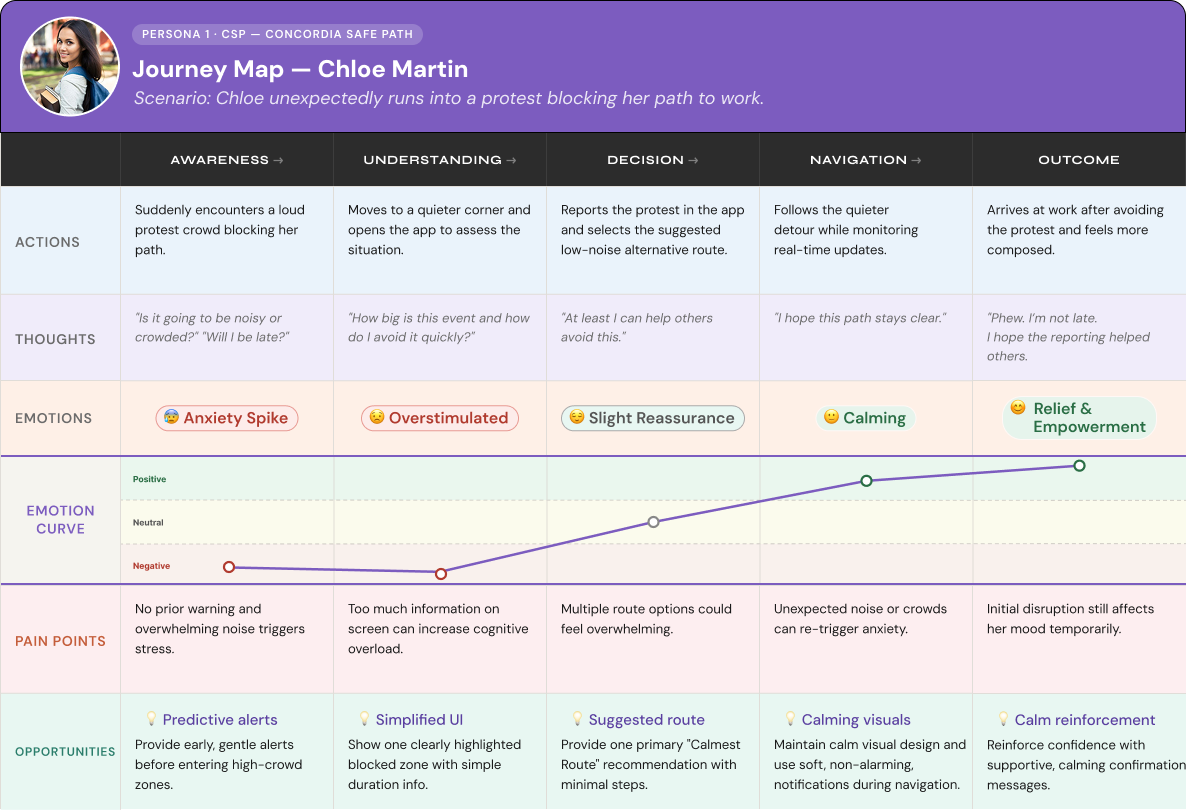
\includegraphics[width=0.9\textwidth, height=0.40\textheight, keepaspectratio]{journey_maps/ChloeMartin_JourneyMap_low.png}
  \captionof{figure}{Journey Map: Chloe Martin. \textit{Scenario: Chloe unexpectedly runs into a protest blocking her path to work near the Hall building.}}
  \label{fig:journey_chloe}
\end{minipage}}
 
\vspace{0.5cm}
 
\noindent\makebox[\textwidth][c]{%
\begin{minipage}{\textwidth}
  \centering
  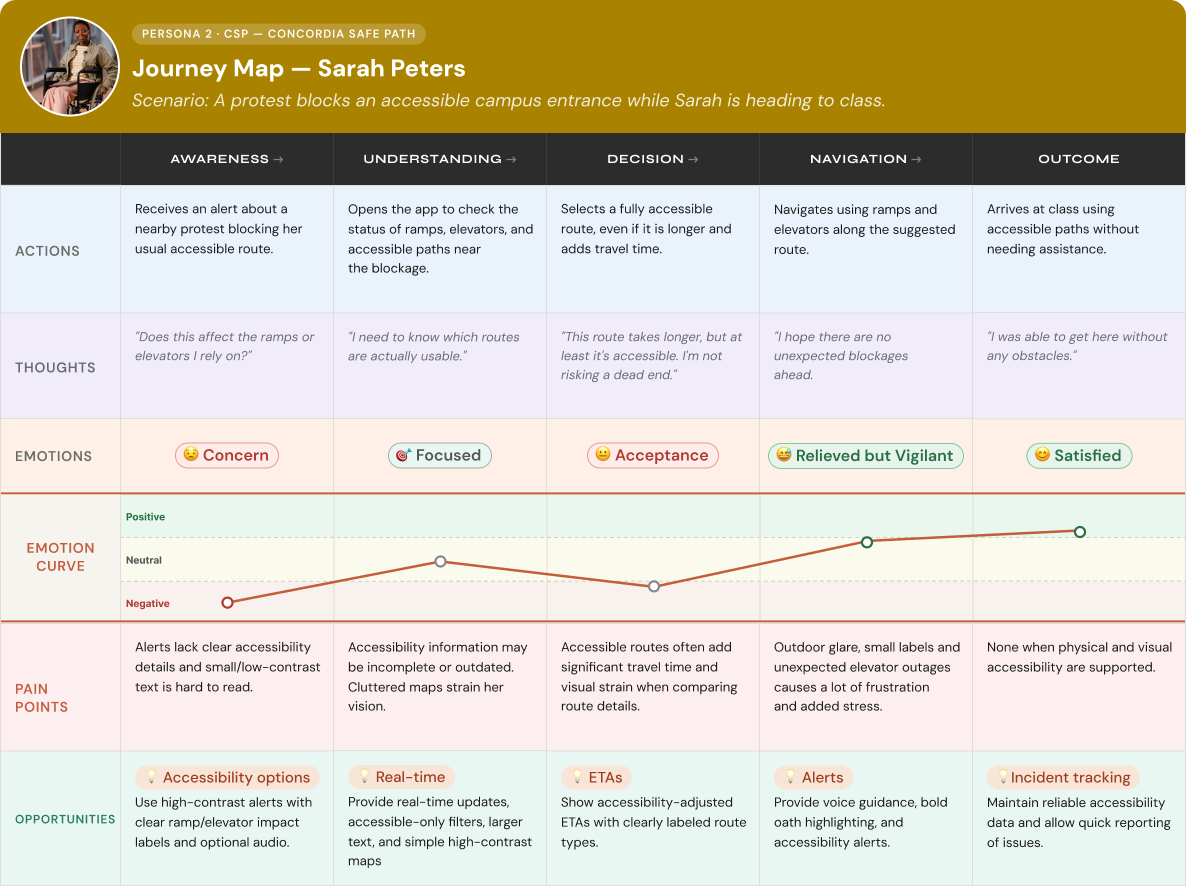
\includegraphics[width=0.9\textwidth, height=0.44\textheight, keepaspectratio]{journey_maps/SarahPeters_JourneyMap_low.png}
  \captionof{figure}{Journey Map: Sarah Peters. \textit{Scenario: A protest blocks an accessible campus entrance while Sarah is heading to class.}}
  \label{fig:journey_sarah}
\end{minipage}}
 
\newpage
 
\noindent\makebox[\textwidth][c]{%
\begin{minipage}{\textwidth}
  \centering
  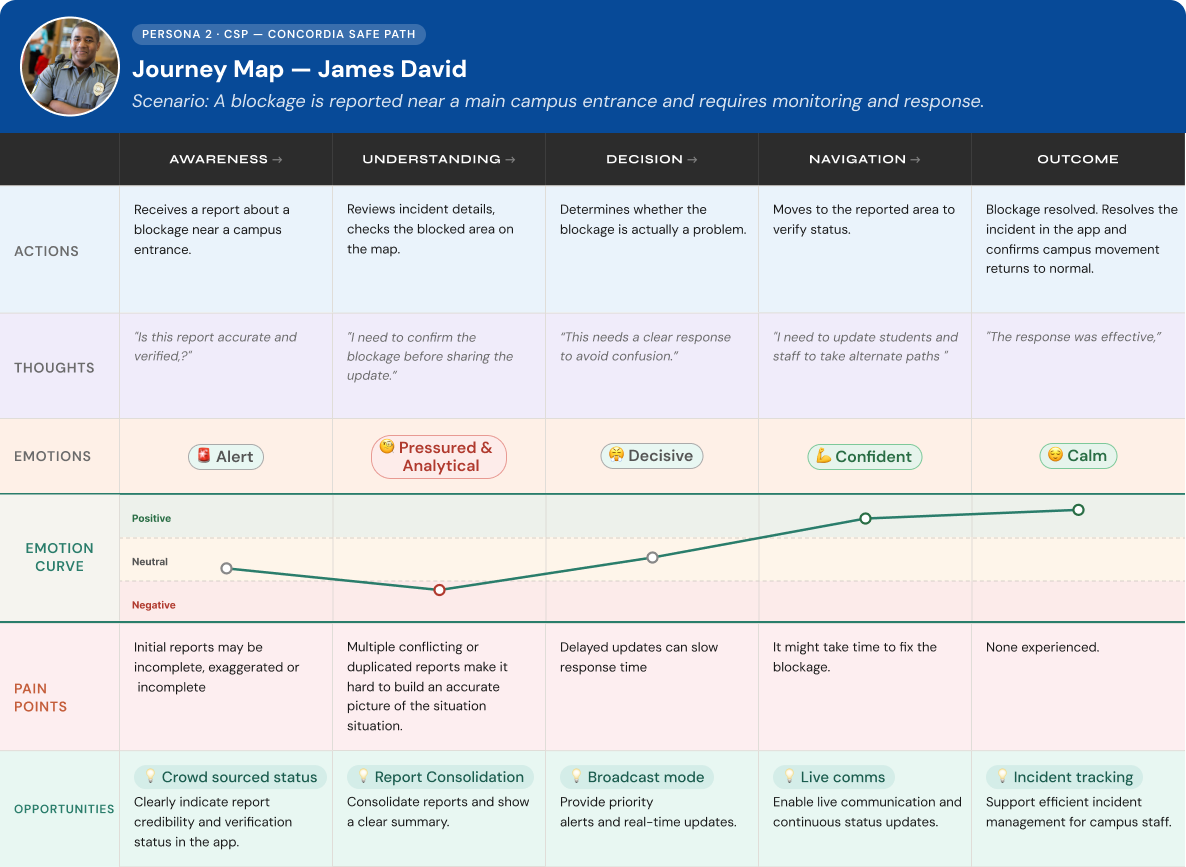
\includegraphics[width=0.8\textwidth, keepaspectratio]{journey_maps/JamesDavid_JourneyMap_low.png}
  \captionof{figure}{Journey Map: James David. \textit{Scenario: A blockage is reported near a main campus entrance and requires monitoring and response.}}
  \label{fig:journey_james}
\end{minipage}}
 
\newpage
 
\section*{Appendix B: Low-Fidelity Wireframes}
\label{appendix:lofi}
 
\noindent\makebox[\textwidth][c]{%
\begin{minipage}{\textwidth}
  \centering
  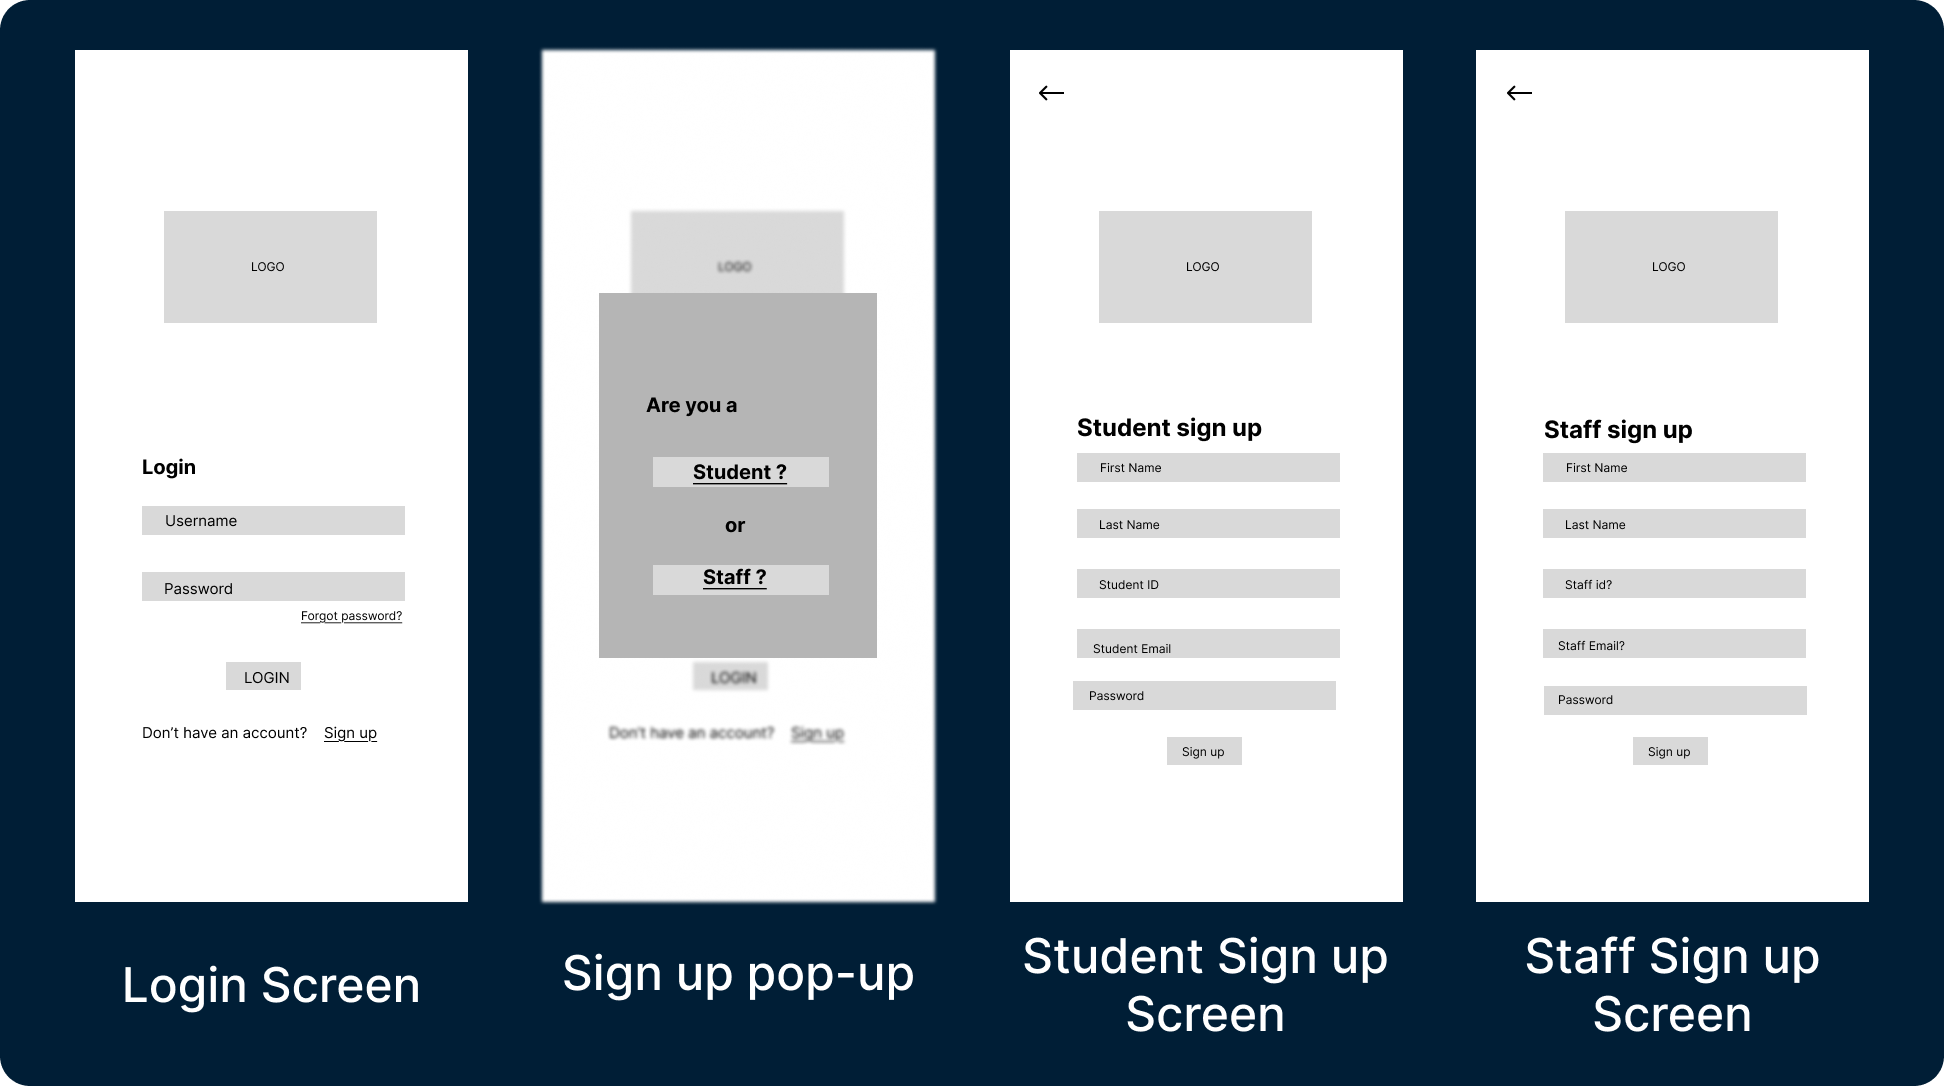
\includegraphics[width=\textwidth, height=0.42\textheight, keepaspectratio]{lofi/Login_Signup_low.png}
  \captionof{figure}{Login / Sign Up low-fidelity designs.}
  \label{fig:lofi_login}
\end{minipage}}
 
\vspace{0.5cm}
 
\noindent\makebox[\textwidth][c]{%
\begin{minipage}{\textwidth}
  \centering
  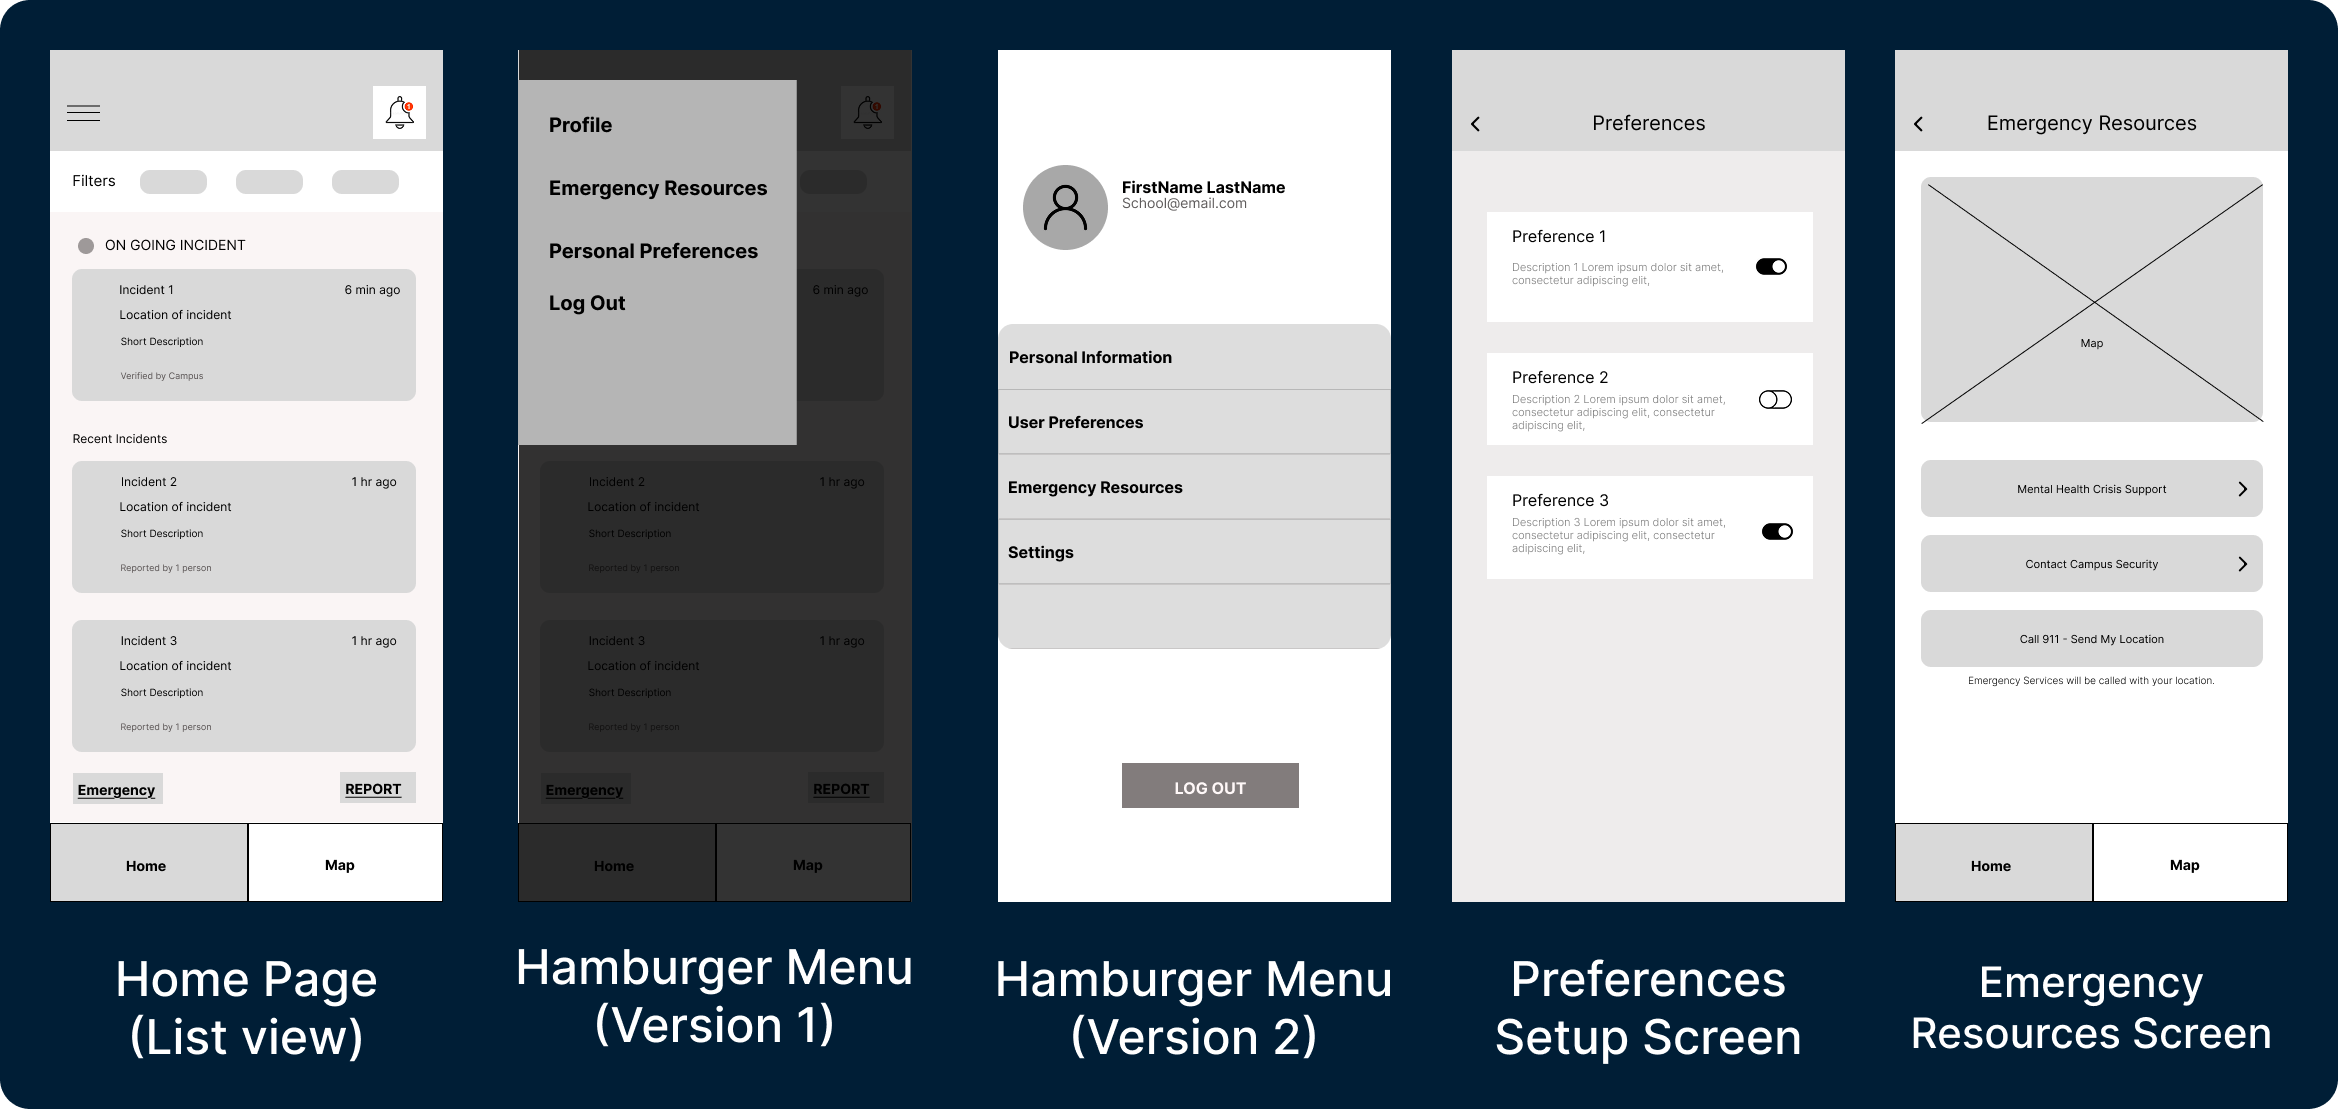
\includegraphics[width=\textwidth, height=0.42\textheight, keepaspectratio]{lofi/Menu_low.png}
  \captionof{figure}{Menu low-fidelity designs.}
  \label{fig:lofi_menu}
\end{minipage}}
 
\newpage
 
\noindent\makebox[\textwidth][c]{%
\begin{minipage}{\textwidth}
  \centering
  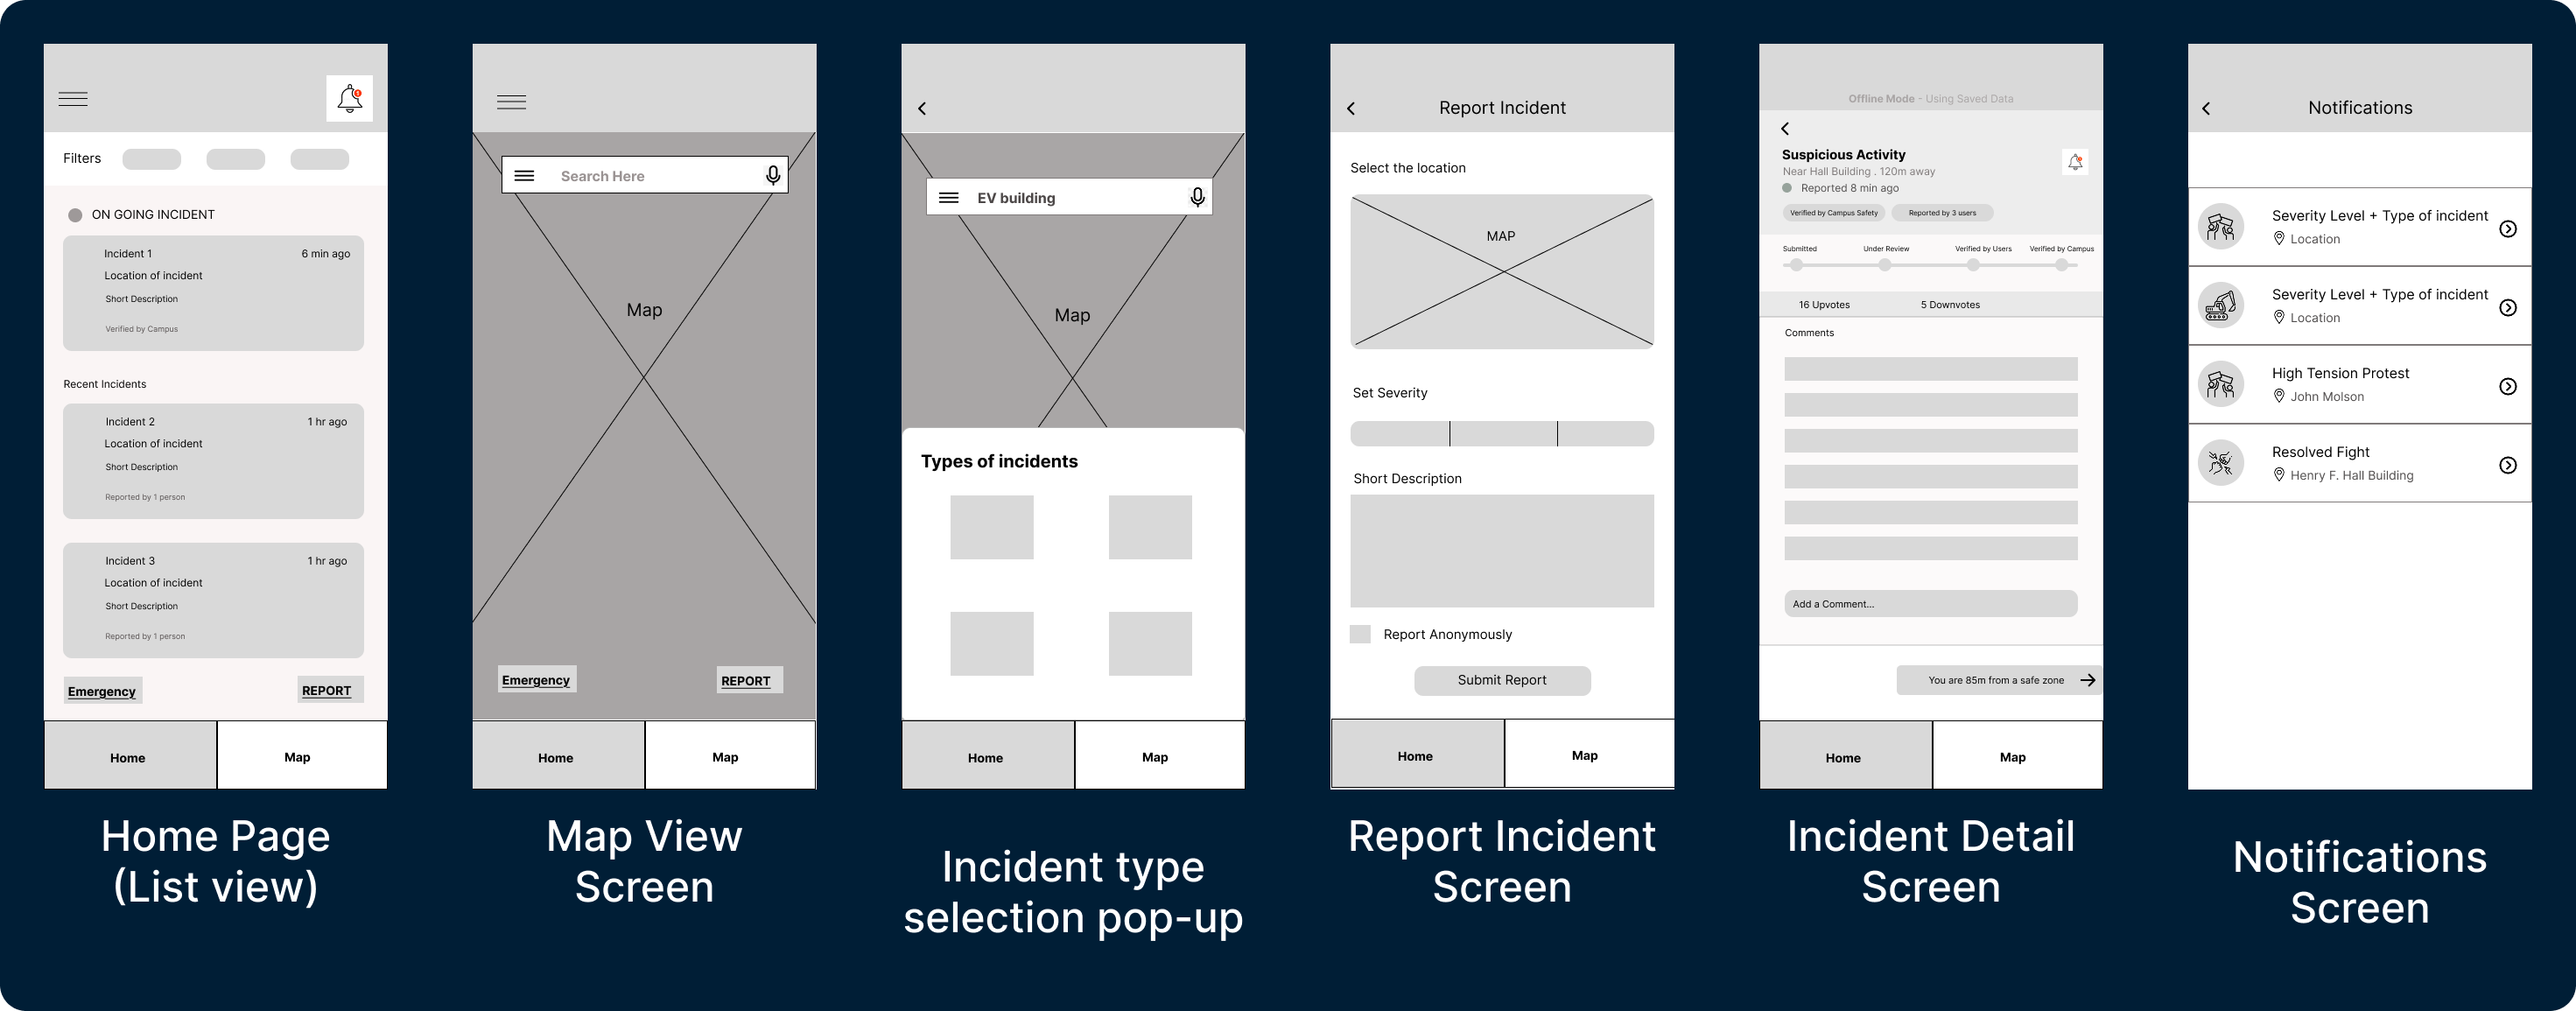
\includegraphics[width=\textwidth, height=0.42\textheight, keepaspectratio]{lofi/Core UI_low.png}
  \captionof{figure}{Core UI views low-fidelity designs.}
  \label{fig:lofi_core}
\end{minipage}}
 
\vspace{0.5cm}
 
\noindent\makebox[\textwidth][c]{%
\begin{minipage}{\textwidth}
  \centering
  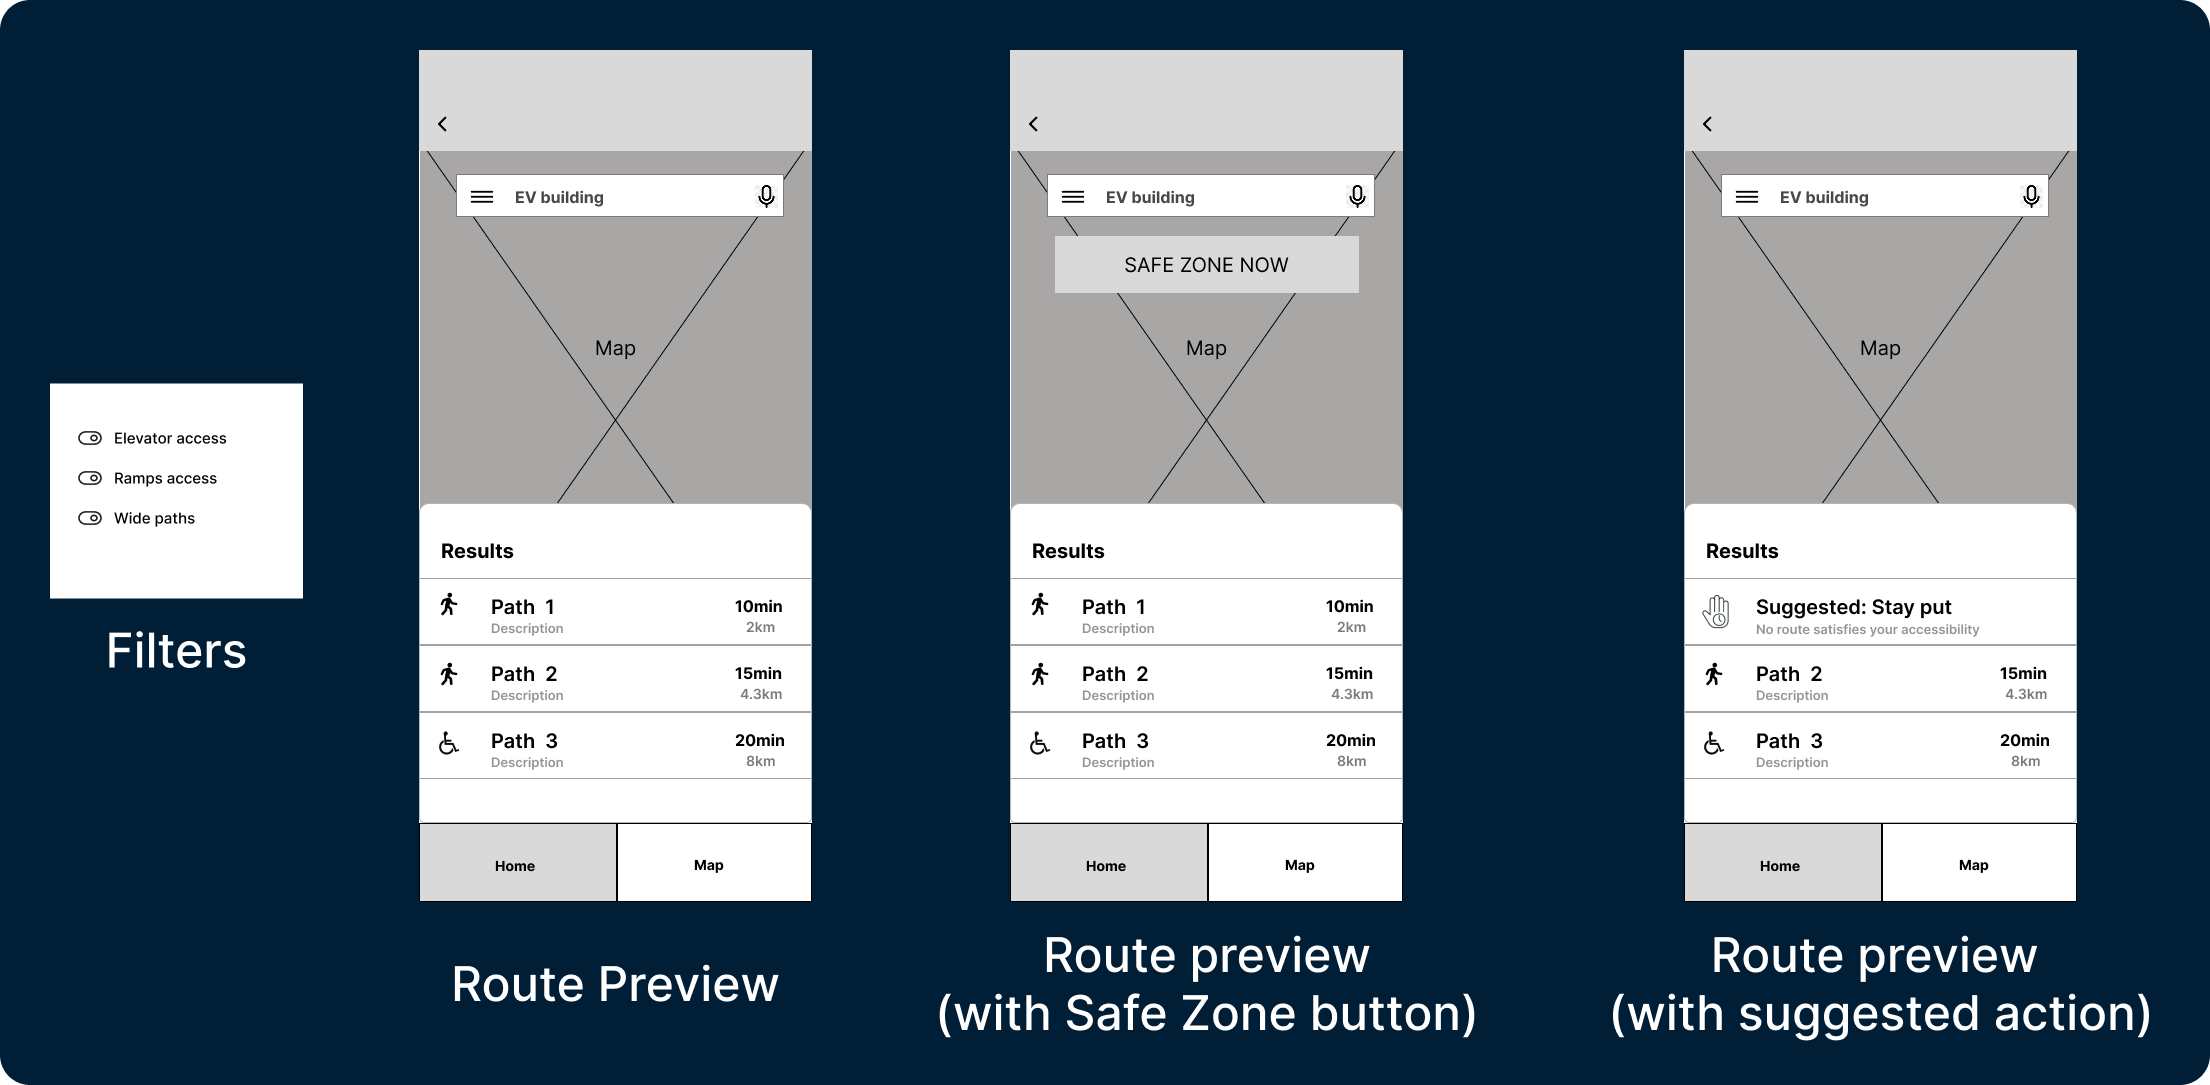
\includegraphics[width=\textwidth, height=0.42\textheight, keepaspectratio]{lofi/Route Planning_low.png}
  \captionof{figure}{Route planning views low-fidelity designs.}
  \label{fig:lofi_route}
\end{minipage}}
 
\newpage
 
\section*{Appendix C: High-Fidelity Prototypes}
\label{appendix:hifi}
 
\noindent\makebox[\textwidth][c]{%
\begin{minipage}{\textwidth}
  \centering
  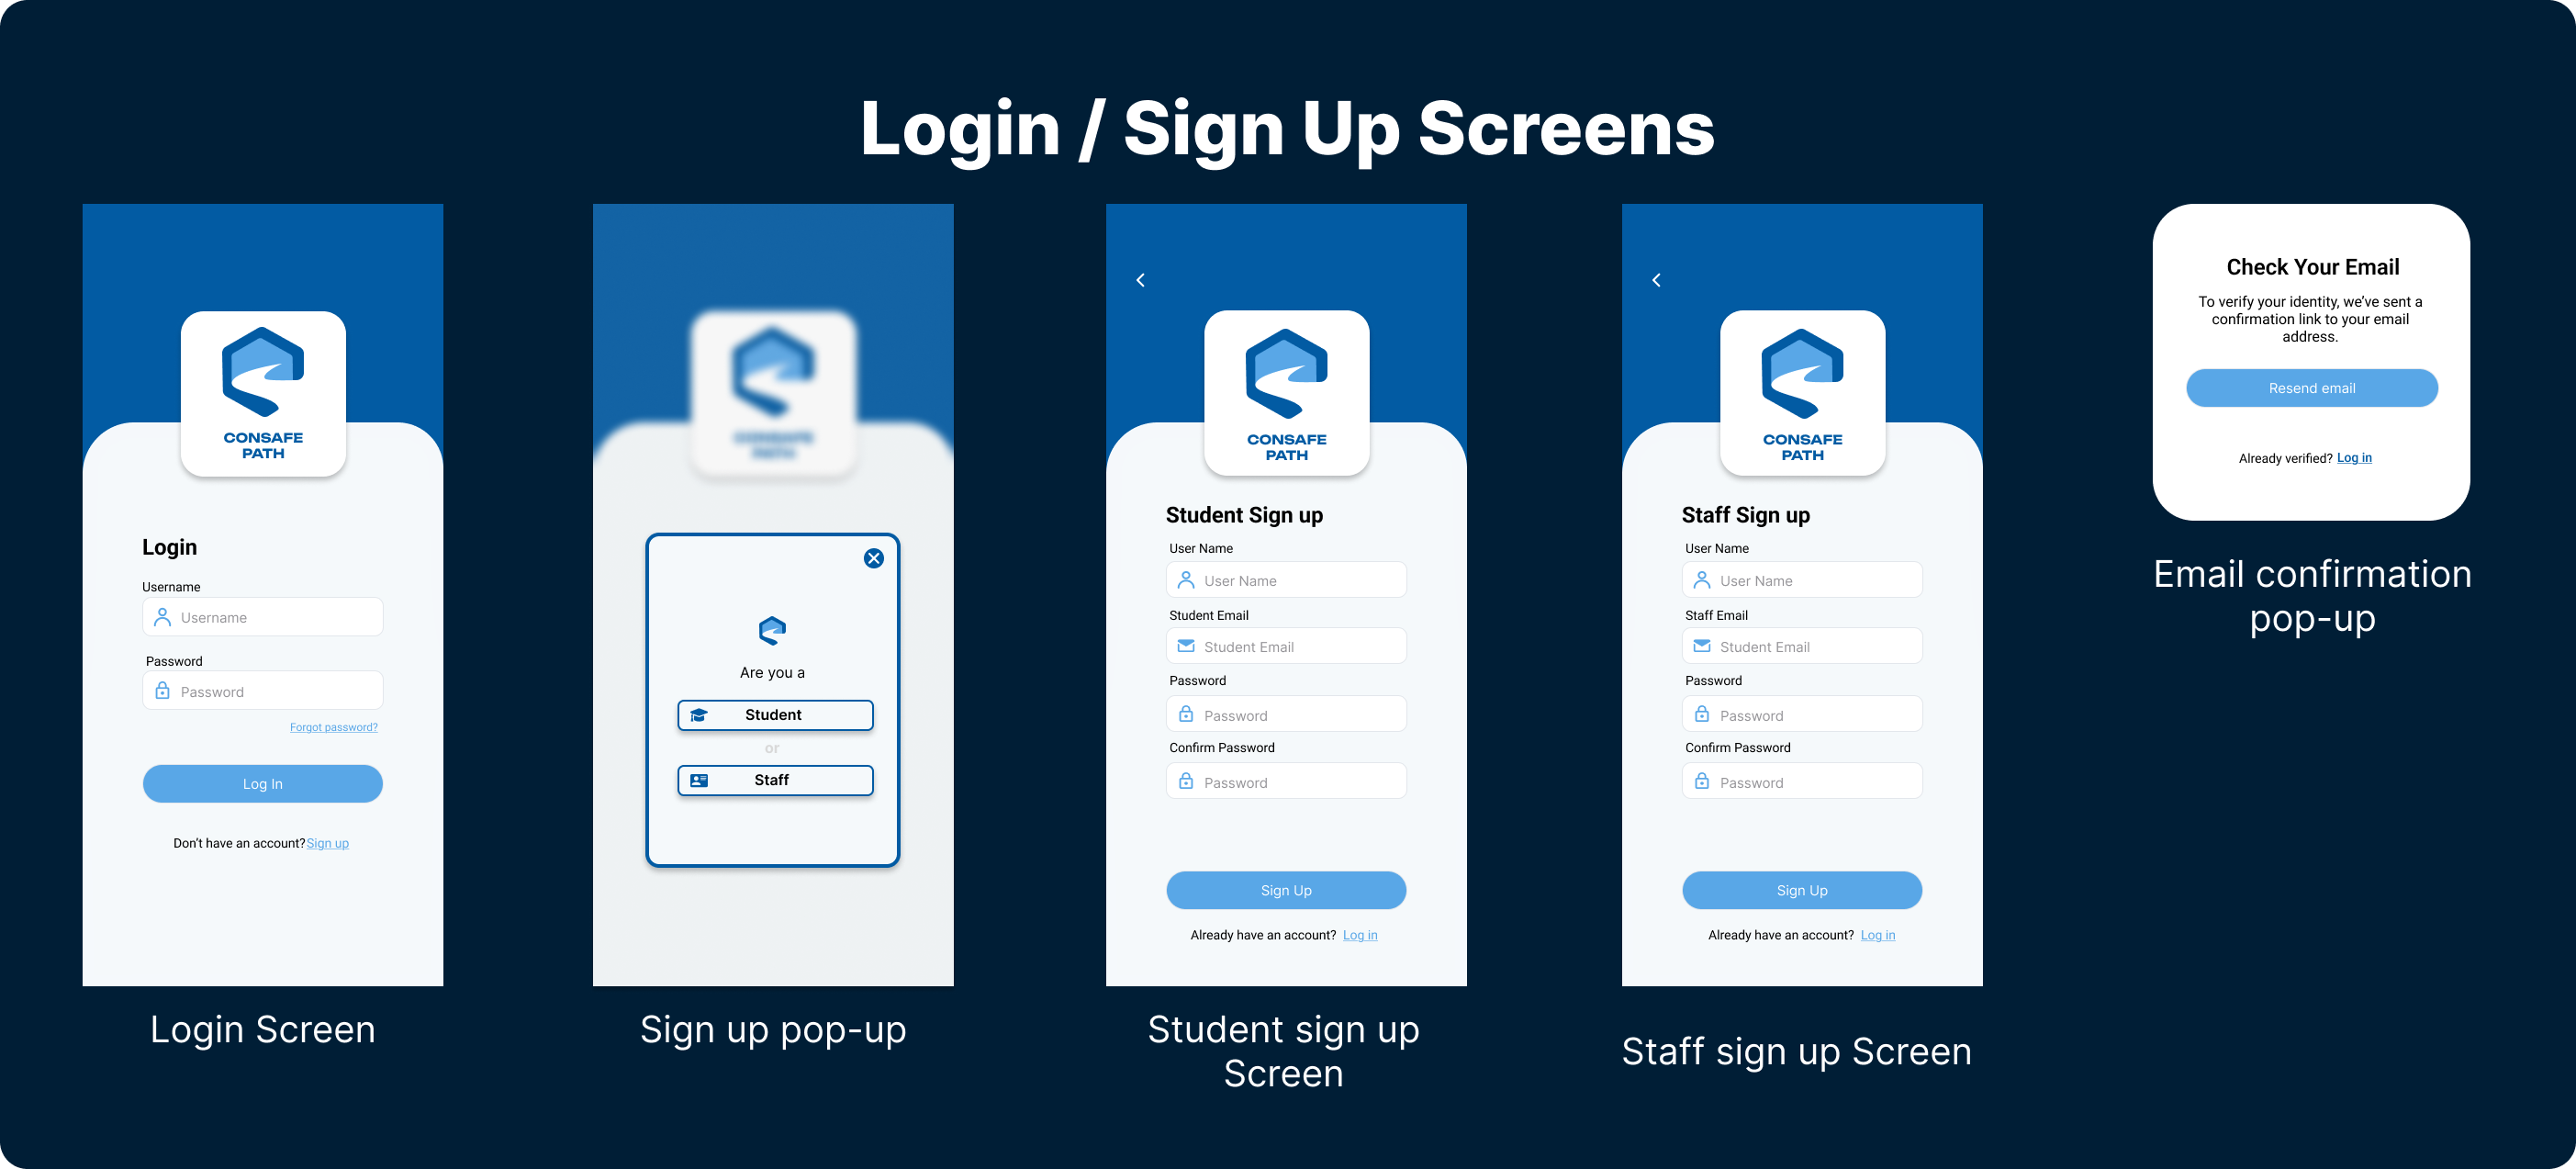
\includegraphics[width=\textwidth, height=0.42\textheight, keepaspectratio]{hifi/LoginSignUp.png}
  \captionof{figure}{Login / Sign Up high-fidelity designs.}
  \label{fig:hifi_login}
\end{minipage}}
 
\vspace{0.5cm}
 
\noindent\makebox[\textwidth][c]{%
\begin{minipage}{\textwidth}
  \centering
  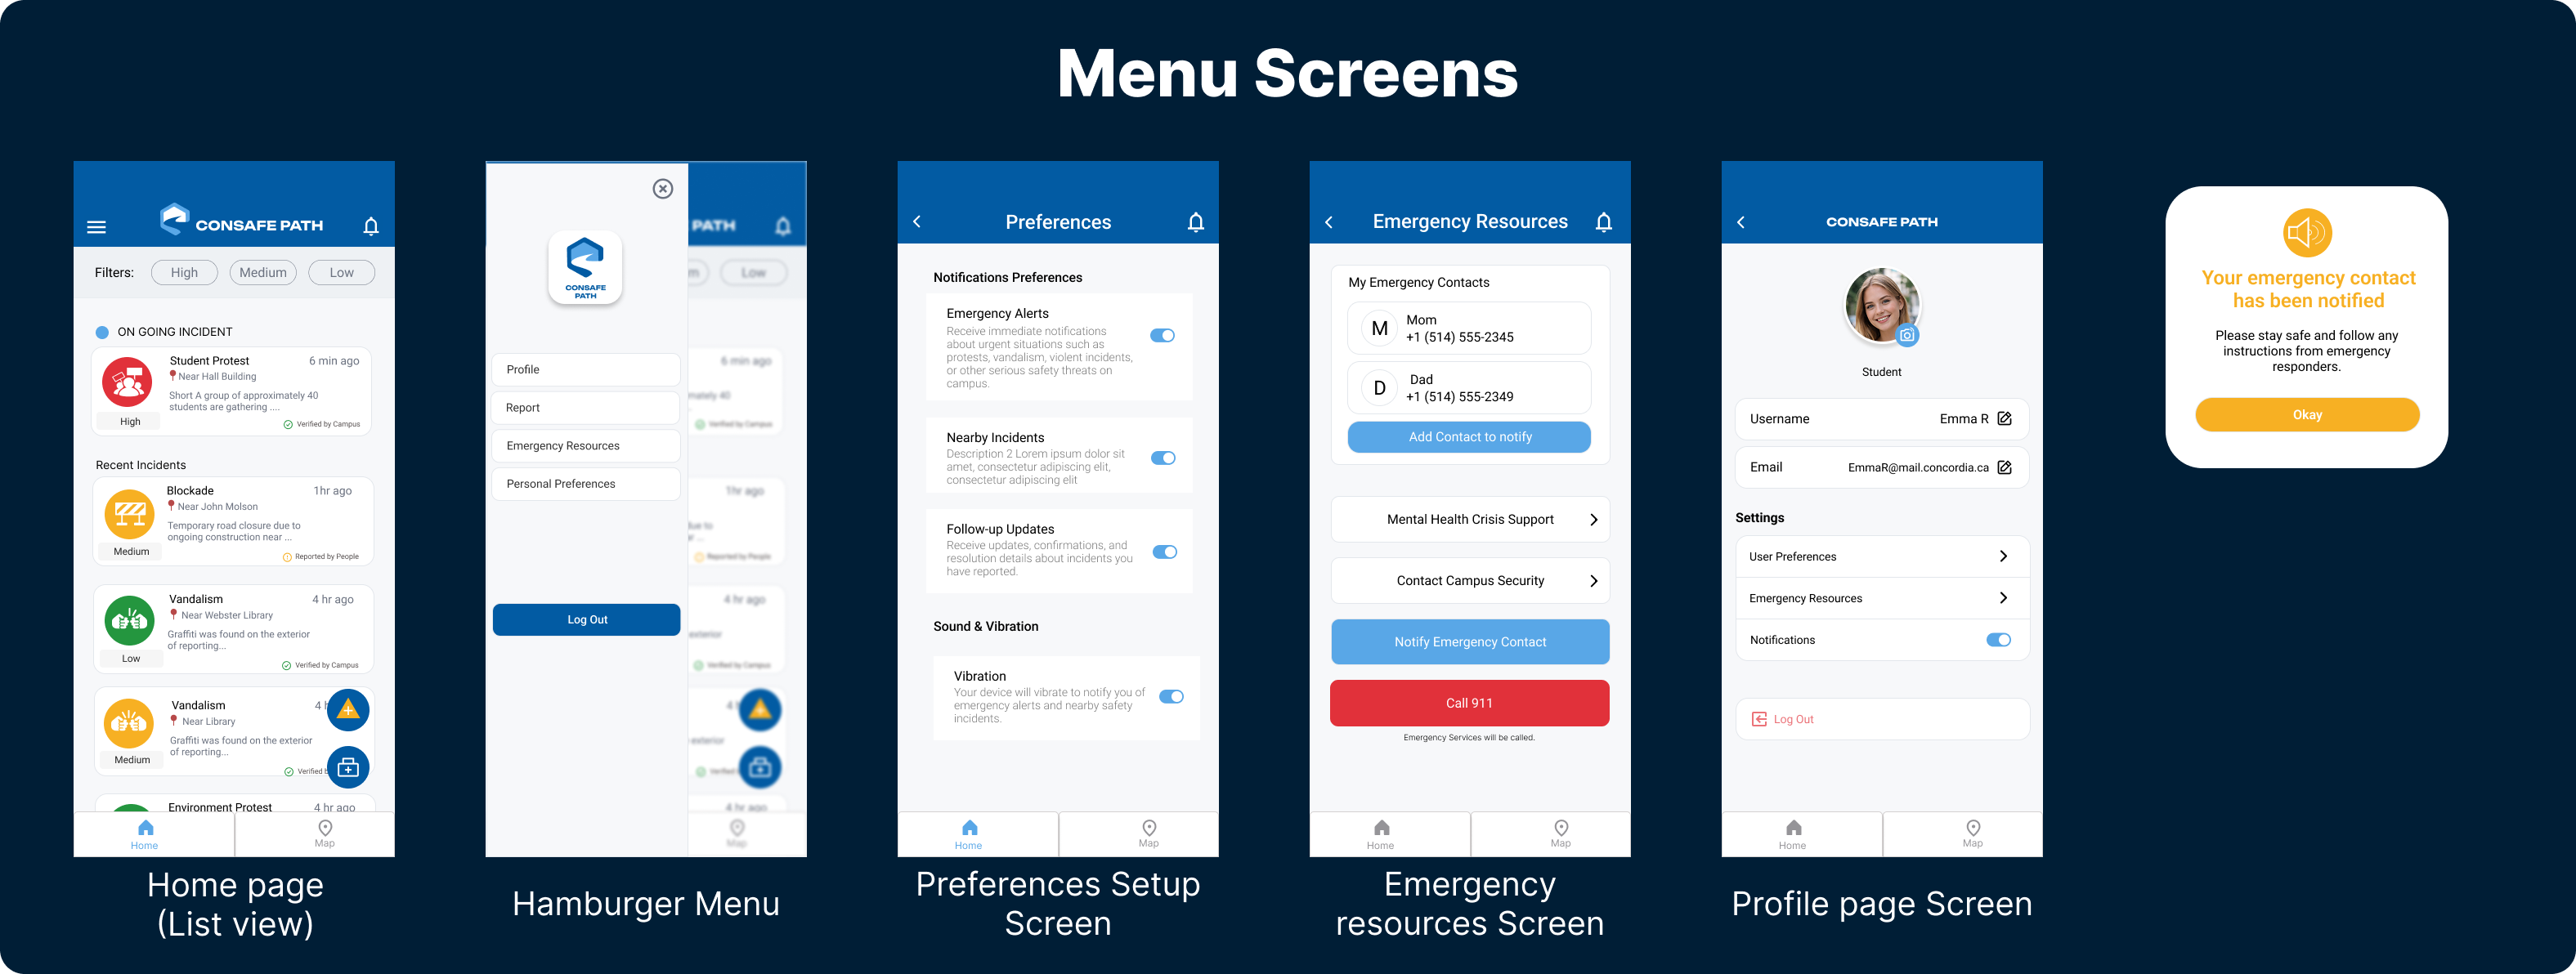
\includegraphics[width=\textwidth, height=0.42\textheight, keepaspectratio]{hifi/Menu.png}
  \captionof{figure}{Menu high-fidelity designs.}
  \label{fig:hifi_menu}
\end{minipage}}
 
\newpage
 
\noindent\makebox[\textwidth][c]{%
\begin{minipage}{\textwidth}
  \centering
  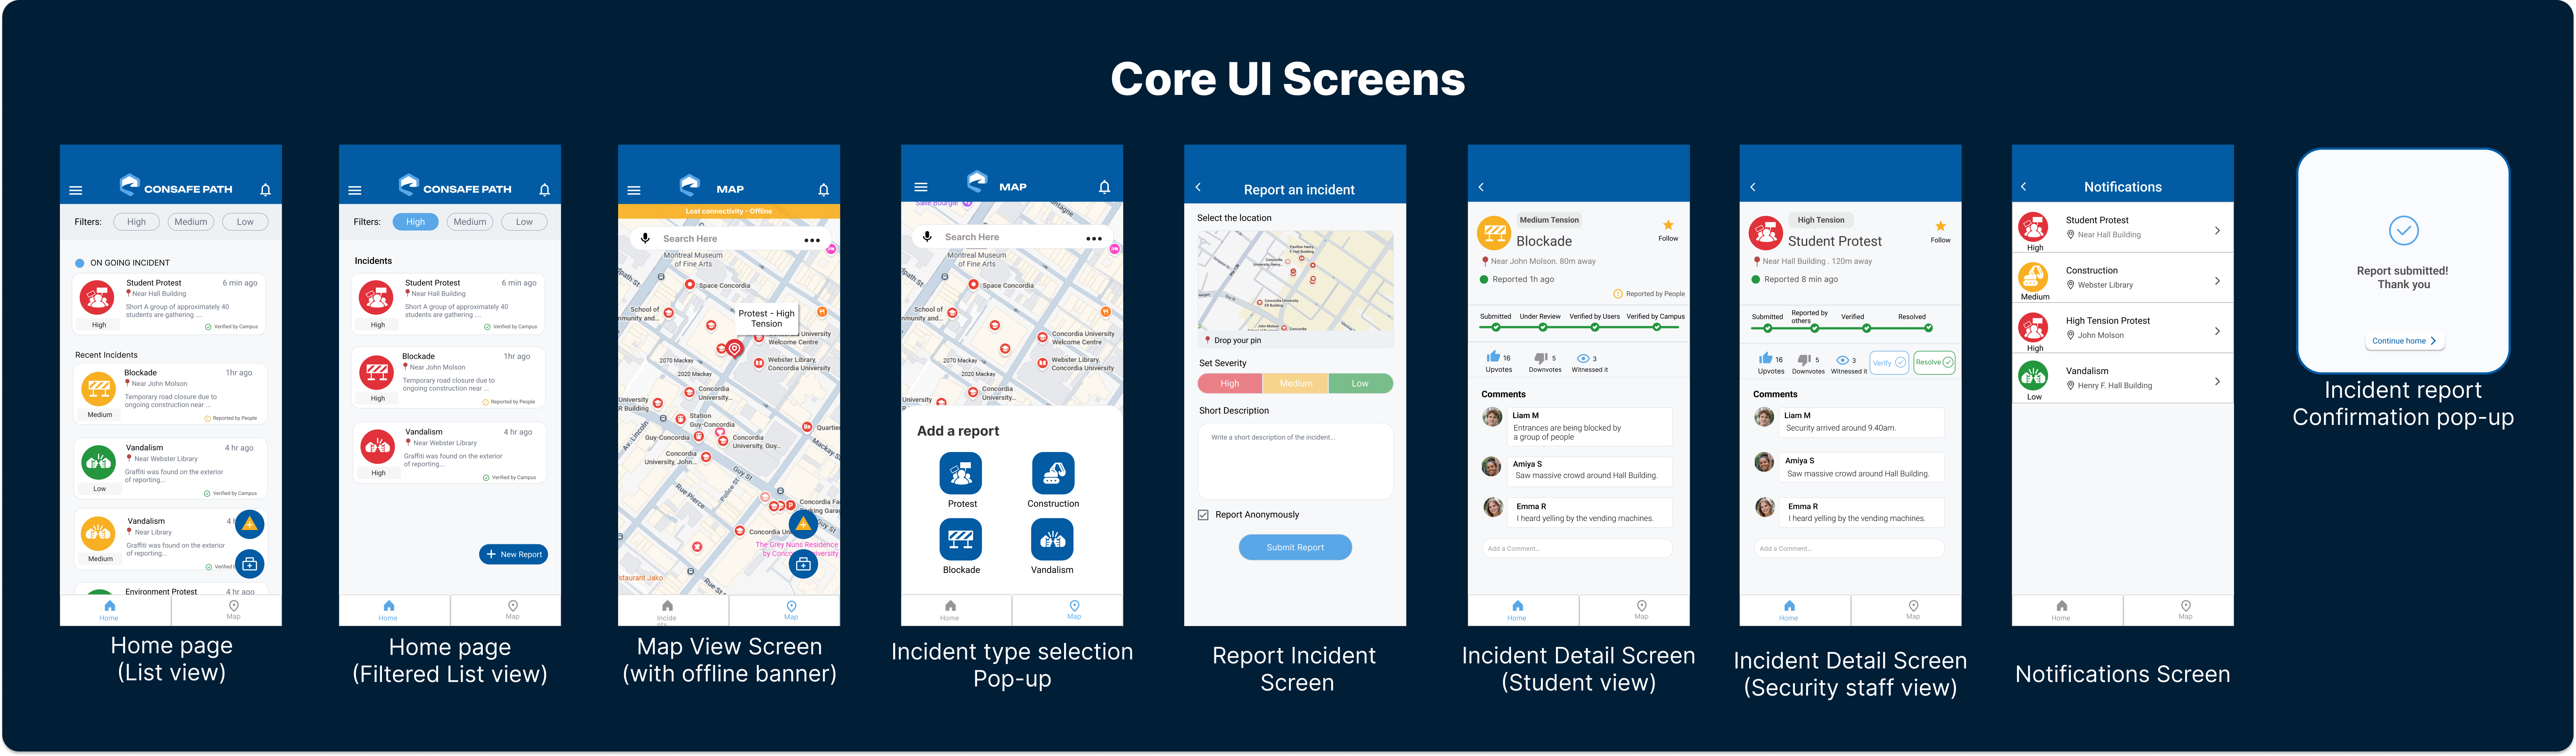
\includegraphics[width=\textwidth, height=0.42\textheight, keepaspectratio]{hifi/Core UI.png}
  \captionof{figure}{Core UI views high-fidelity designs.}
  \label{fig:hifi_core}
\end{minipage}}
 
\vspace{0.5cm}
 
\noindent\makebox[\textwidth][c]{%
\begin{minipage}{\textwidth}
  \centering
  
\includegraphics[width=\textwidth, height=0.42\textheight, keepaspectratio]{hifi/Route Planning.png}
  \captionof{figure}{Route planning high-fidelity designs.}
  \label{fig:hifi_route}
\end{minipage}}
 
\newpage
 
\section*{Appendix D: Heuristic Evaluation}
\label{appendix:heuristics}
 
\noindent\makebox[\textwidth][c]{%
\begin{minipage}{\textwidth}
\centering
\renewcommand{\arraystretch}{1.3}
\setlength{\tabcolsep}{4pt}
\captionof{table}{Heuristic evaluation of CSP screens against Nielsen's 10 Usability Heuristics. Y~=~Yes, P~=~Partial, N~=~No, --~=~Not applicable.}
\label{tab:heuristics}
\begin{tabular}{|M{0.16\linewidth}|c|c|c|c|c|c|c|c|c|c|}
\hline
\rowcolor{tableheader}
\textcolor{white}{\textbf{Screen}}
  & \textcolor{white}{\textbf{\rotatebox{70}{Visibility}}}
  & \textcolor{white}{\textbf{\rotatebox{70}{Mapping}}}
  & \textcolor{white}{\textbf{\rotatebox{70}{User Control}}}
  & \textcolor{white}{\textbf{\rotatebox{70}{Consistency}}}
  & \textcolor{white}{\textbf{\rotatebox{70}{Error Prevention}}}
  & \textcolor{white}{\textbf{\rotatebox{70}{Recognition}}}
  & \textcolor{white}{\textbf{\rotatebox{70}{Flexibility}}}
  & \textcolor{white}{\textbf{\rotatebox{70}{Aesthetics}}}
  & \textcolor{white}{\textbf{\rotatebox{70}{Error Recovery}}}
  & \textcolor{white}{\textbf{\rotatebox{70}{Help \& Docs}}} \\
\hline
\rowcolor{tablerowA}
Sign Up        & Y & Y & Y & Y & Y & Y & Y & Y & Y & P \\
\hline
\rowcolor{tablerowB}
Login          & Y & Y & Y & Y & Y & Y & Y & Y & P & P \\
\hline
\rowcolor{tablerowA}
Profile        & P & Y & Y & Y & Y & Y & P & Y & Y & Y \\
\hline
\rowcolor{tablerowB}
Preferences    & Y & Y & Y & Y & P & Y & Y & Y & Y & Y \\
\hline
\rowcolor{tablerowA}
Emergency      & Y & Y & Y & Y & Y & Y & Y & Y & Y & Y \\
\hline
\rowcolor{tablerowB}
Incidents List & Y & Y & P & Y & Y & Y & P & Y & Y & -- \\
\hline
\rowcolor{tablerowA}
Incident Detail & Y & Y & P & Y & Y & Y & Y & Y & N & -- \\
\hline
\rowcolor{tablerowB}
Report Incident & Y & Y & N & Y & Y & Y & P & Y & P & -- \\
\hline
\rowcolor{tablerowA}
Map            & Y & Y & Y & Y & Y & P & P & Y & Y & -- \\
\hline
\rowcolor{tablerowB}
Notifications  & P & Y & N & Y & P & Y & P & Y & Y & N \\
\hline
\end{tabular}
\end{minipage}}

\newpage
 
\section*{Appendix E: User Flow Diagrams}
\label{appendix:userflows}
 
\noindent\makebox[\textwidth][c]{%
\begin{minipage}{\textwidth}
  \centering
  
\includegraphics[width=\textwidth, keepaspectratio]{user_flows/Login_Signup_low.png}
  \captionof{figure}{Login / Sign Up user flow.}
  \label{fig:flow_login}
\end{minipage}}
 
\vspace{0.5cm}
 
\noindent\makebox[\textwidth][c]{%
\begin{minipage}{\textwidth}
  \centering
  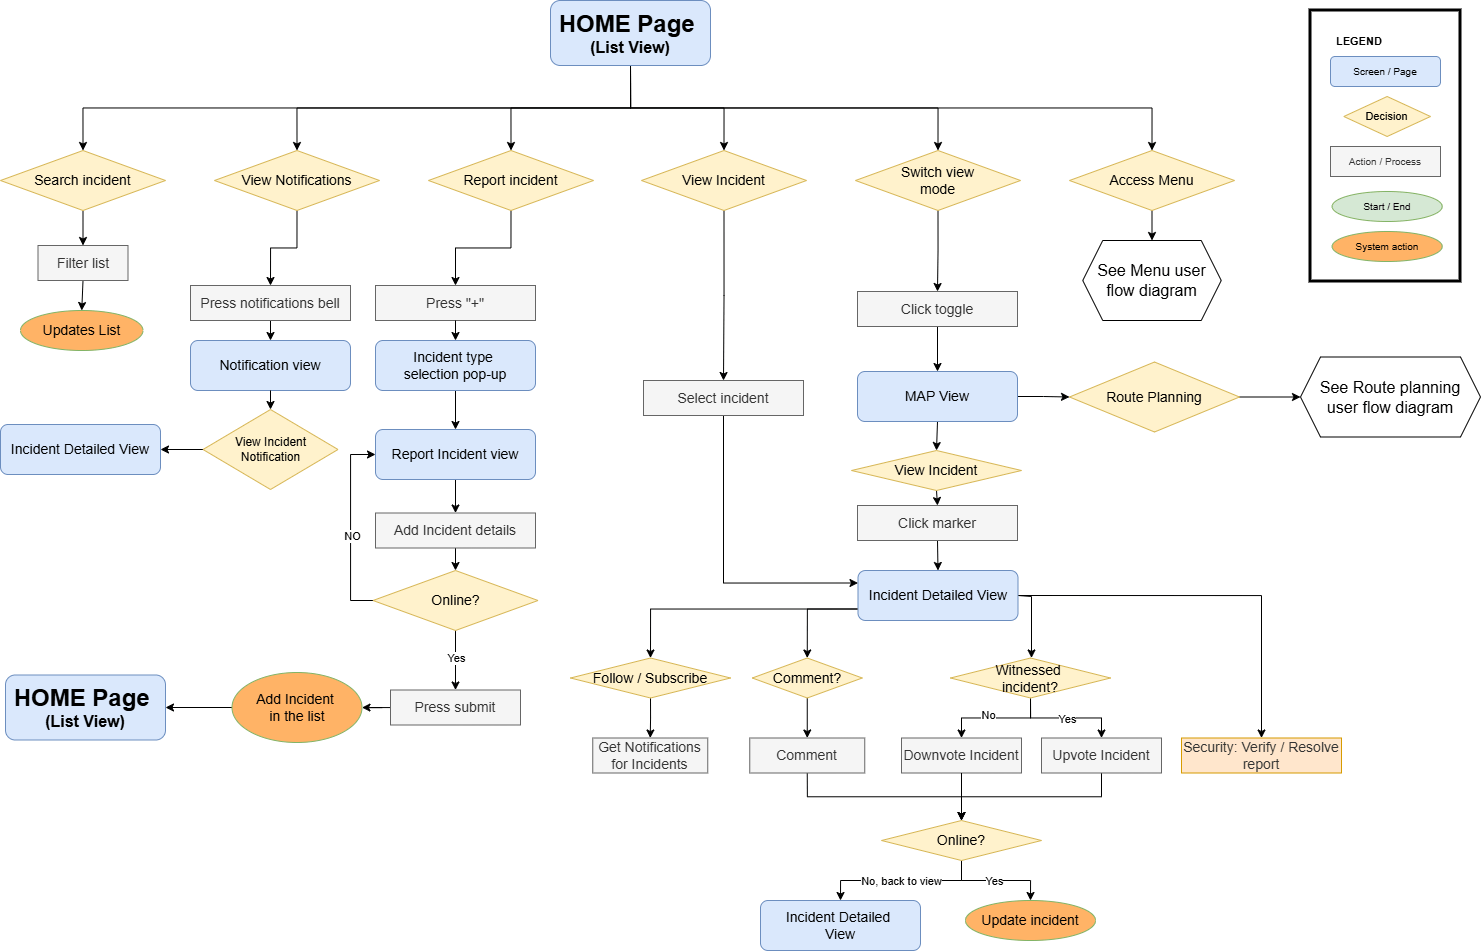
\includegraphics[width=\textwidth, keepaspectratio]{user_flows/CoreUI_low.png}
  \captionof{figure}{UI navigation user flow.}
  \label{fig:flow_navigation}
\end{minipage}}
 
\newpage
 
\noindent\makebox[\textwidth][c]{%
\begin{minipage}{\textwidth}
  \centering
  
\includegraphics[width=\textwidth, keepaspectratio]{user_flows/Menu_low.png}
  \captionof{figure}{Menu user flow.}
  \label{fig:flow_menu}
\end{minipage}}
 
\vspace{0.5cm}
 
\noindent\makebox[\textwidth][c]{%
\begin{minipage}{\textwidth}
  \centering
  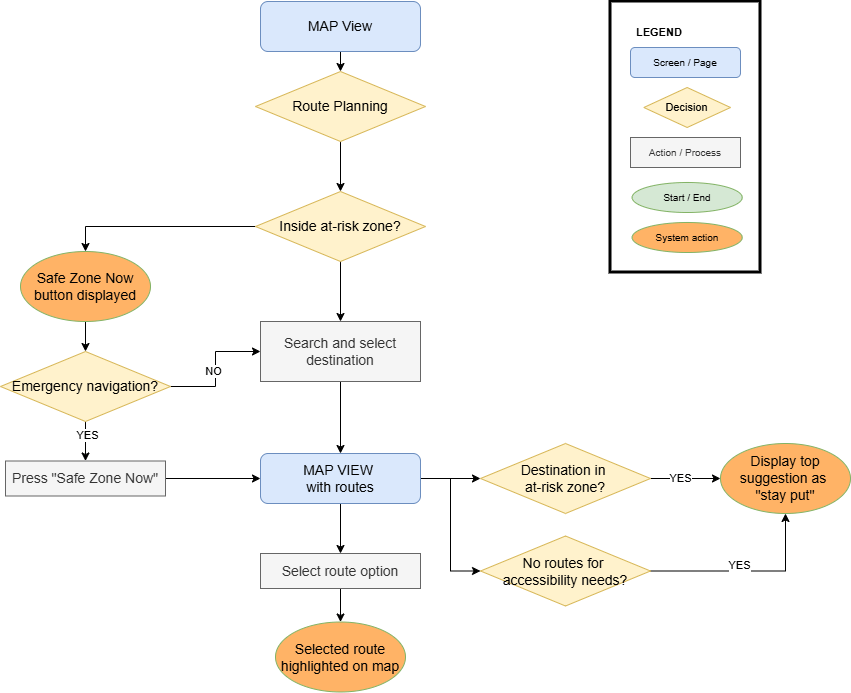
\includegraphics[width=\textwidth, keepaspectratio]{user_flows/RoutePlanning_low.png}
  \captionof{figure}{Route planning user flow.}
  \label{fig:flow_route}
\end{minipage}}

\end{document}
\endinput